\documentclass{beamer}
\usepackage[italian]{babel}
\usepackage[utf8]{inputenc}
\usepackage[T1]{fontenc}
\usepackage{graphicx}
\usepackage{tikz}
\usepackage{booktabs}
\usepackage{hyperref}
\usepackage{eurosym}
\usepackage{subfig}
\usepackage{textpos}


\usetheme{AnnArbor}
%\useoutertheme{miniframes}
\setbeamercovered{dynamic}


\institute[DICAM - UNITN]{\normalsize{Universit\`a degli Studi di Trento}\\\footnotesize{Dipartimento di ingegneria civile, ambientale e meccanica\\Laurea Magistrale in Ingegneria Civile\\ Anno Accademico 2018/2019}}
\logo{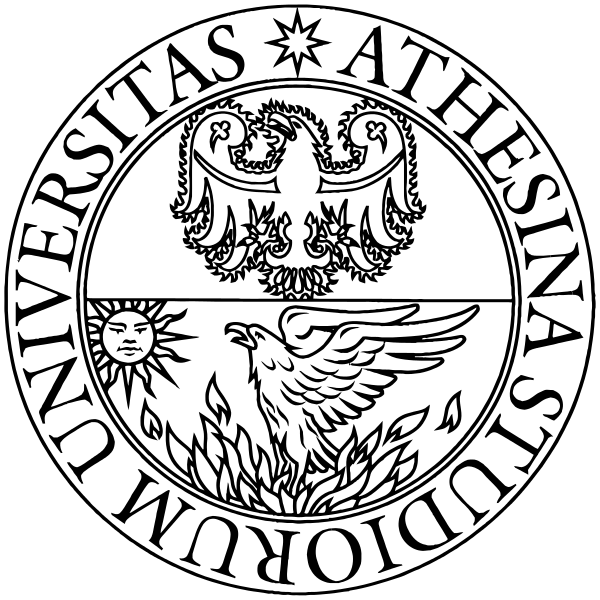
\includegraphics[width = 15mm]{images/logo}}

\title[Progetto di un acquedotto]{Progetto di un acquedotto a Pergine Valsugana}
\subtitle{Corso di Costruzioni Idrauliche}

\author[Franzoi - Rebellato]{%
  \texorpdfstring{%
    \begin{columns}
      \column{.3333\linewidth}
      \centering
      \textbf{Studenti}: \\  Matteo Franzoi \\ Andrea Rebellato
      \column{.3333\linewidth}
      \centering
      \textbf{Docente}: \\ Prof. Riccardo Rigon
       \column{.3333\linewidth}
      \centering
        \textbf{Esercitatori}: \\ Niccolò Tubini \\ Daniele Della Torre
    \end{columns}
}%
 {}%
}%
\date{giugno 2019}
%
%
%
\setbeamertemplate{background canvas}{%
\begin{tikzpicture}[remember picture,overlay]
\shade[top color=gray, bottom color=white]
  (current page.north west)
     rectangle
  (current page.south east);
\end{tikzpicture}%     
}
\setbeamertemplate{navigation symbols}{}

\newcommand{\nologo}{\setbeamertemplate{logo}{}}
%
%
%
\begin{document}
{%
\usebackgroundtemplate{%
 \tikz \node[opacity=.5] {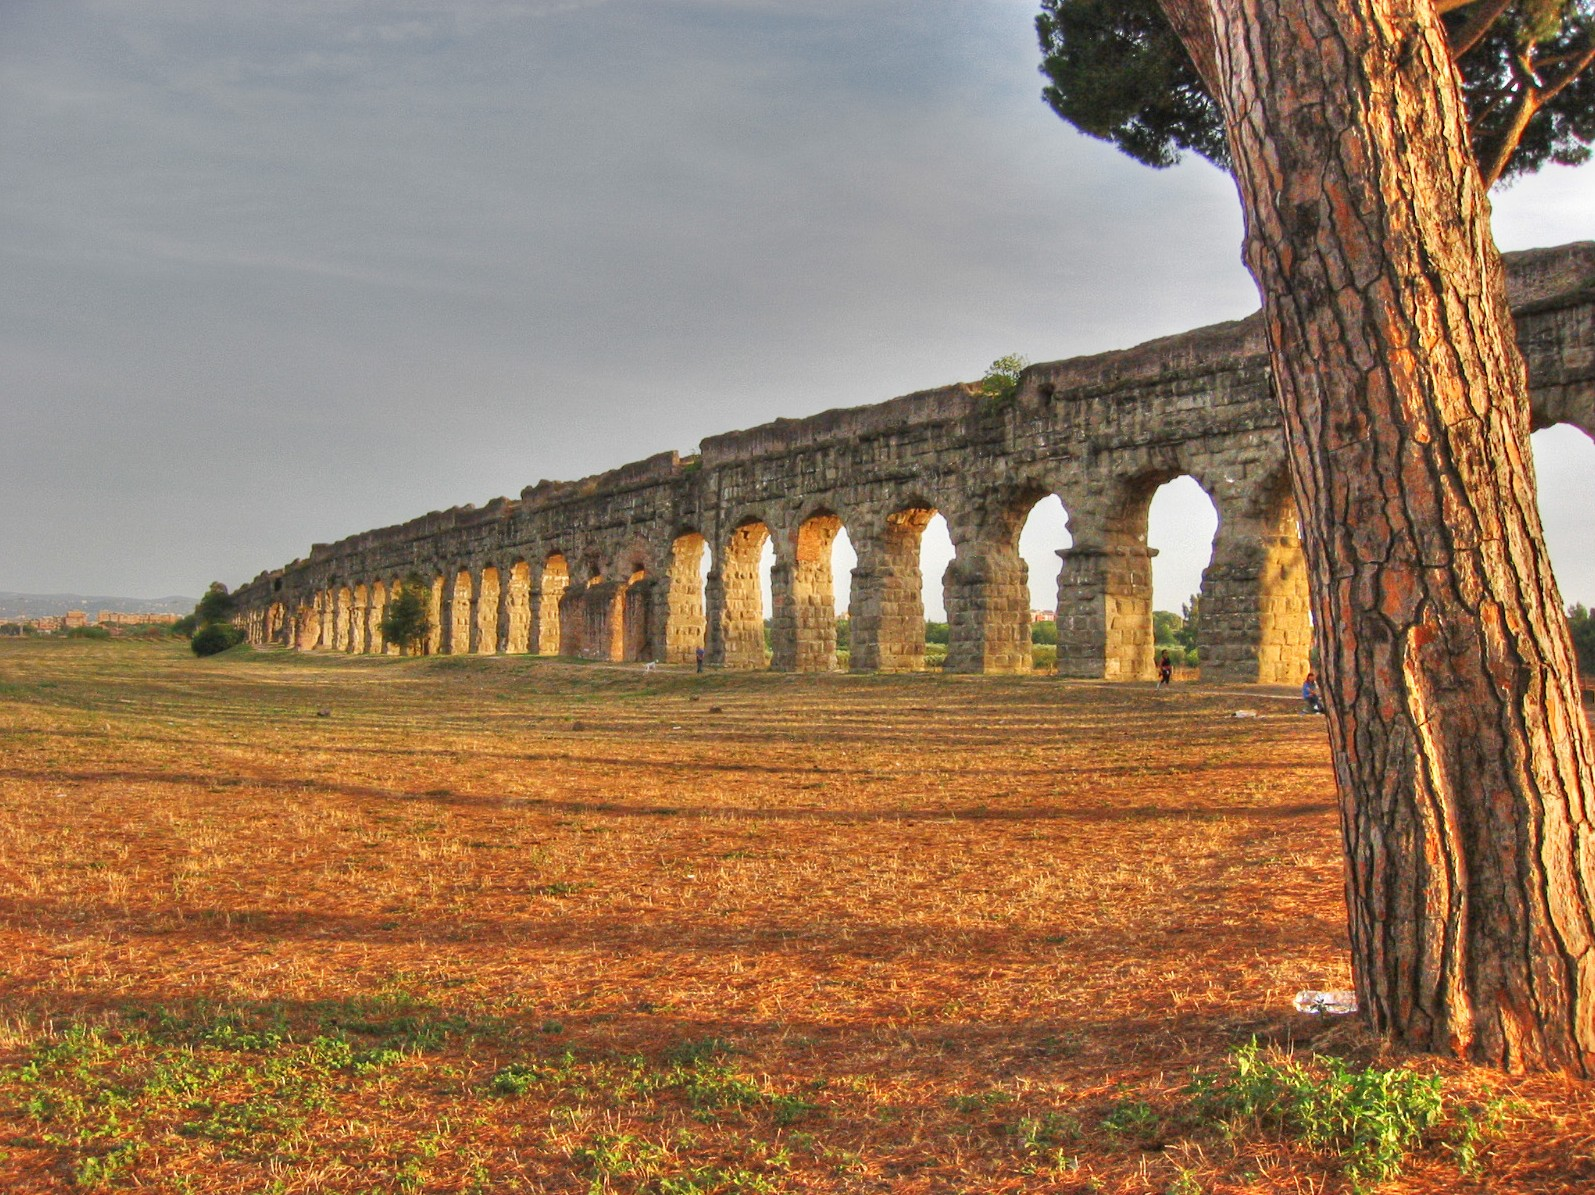
\includegraphics[height=1\paperheight, width=\paperwidth]{images/acquedotto_romani}};
}
\begin{frame}
    \maketitle
\end{frame}
}

\begin{frame}
    \frametitle{Indice}
    \tableofcontents
\end{frame}



\section{Inquadramento}
\begin{frame}
 \frametitle{Scelta dell'area}
 \begin{columns}
 \begin{column}{.5\textwidth}
  \begin{figure}
   \centering
   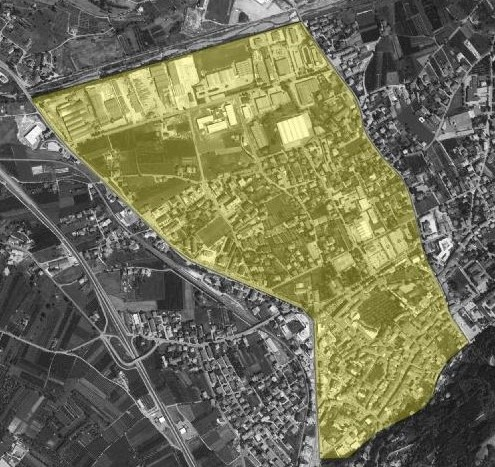
\includegraphics[width=\linewidth]{images/area}
  \end{figure}
  \end{column}

 \begin{column}{.5\textwidth}
  \begin{itemize}[<+->]
   \item Pergine Valsugana, nei pressi di Ponte Regio
   \item a lato del torrente Fersina
   \item parte dell'area in comune con il progetto della fognatura pluviale
   \item superficie di $1.05\,km^2$
  \end{itemize}
 \end{column}
 \end{columns}
 
\end{frame}

\begin{frame}
 \frametitle{Analisi delle aree omogenee}
 
 \begin{columns}
  \begin{column}{.5\textwidth}
   \begin{figure}
    \centering
    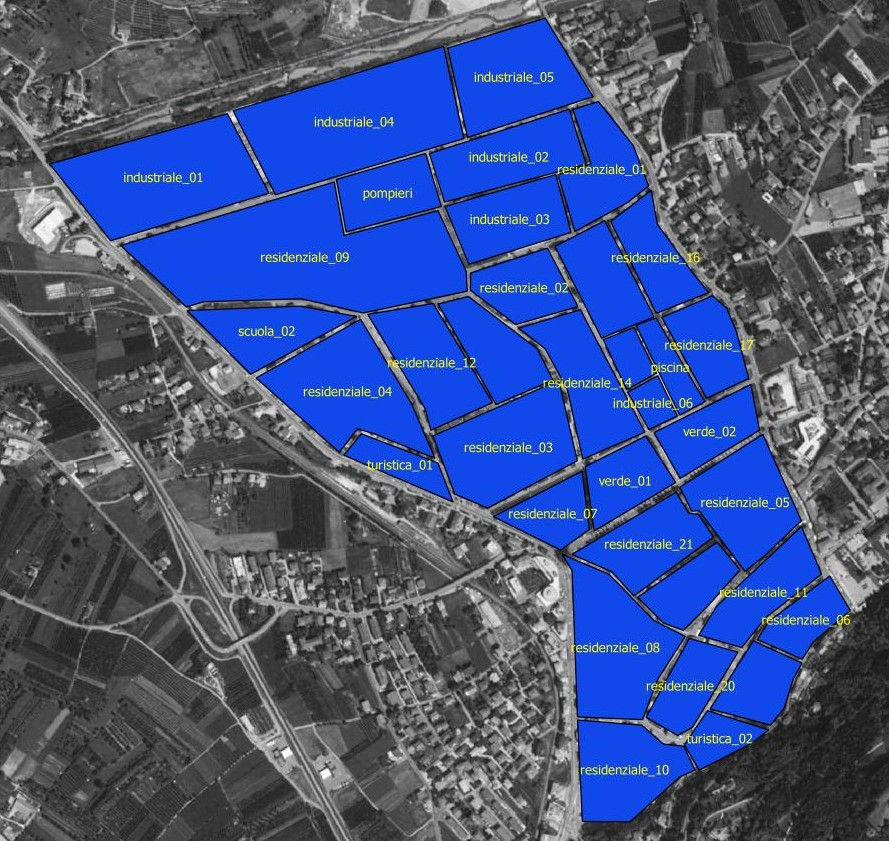
\includegraphics[width=\linewidth]{images/analisi_area}
   \end{figure}
  \end{column}
  
  \begin{column}{.5\textwidth}
   \begin{itemize}[]
    \item divisione della zona nelle principali aree omogenee:
    \begin{itemize}[]
     \item residenziale
     \item turistica
     \item industriale
     \item verde
    \end{itemize}
    \item ulteriore analisi per aree particolari quali:
    \begin{itemize}
     \item poli scolastici
     \item piscina comunale
     \item caserma dei vigili del fuoco permanenti
    \end{itemize}
   \end{itemize}
  \end{column}
 \end{columns} 
\end{frame}

\begin{frame}
 \frametitle{Sorgenti}
 \begin{columns}
    \begin{column}{.5\textwidth}
     \begin{figure}
      \centering
      \begin{overprint}
       \onslide<1>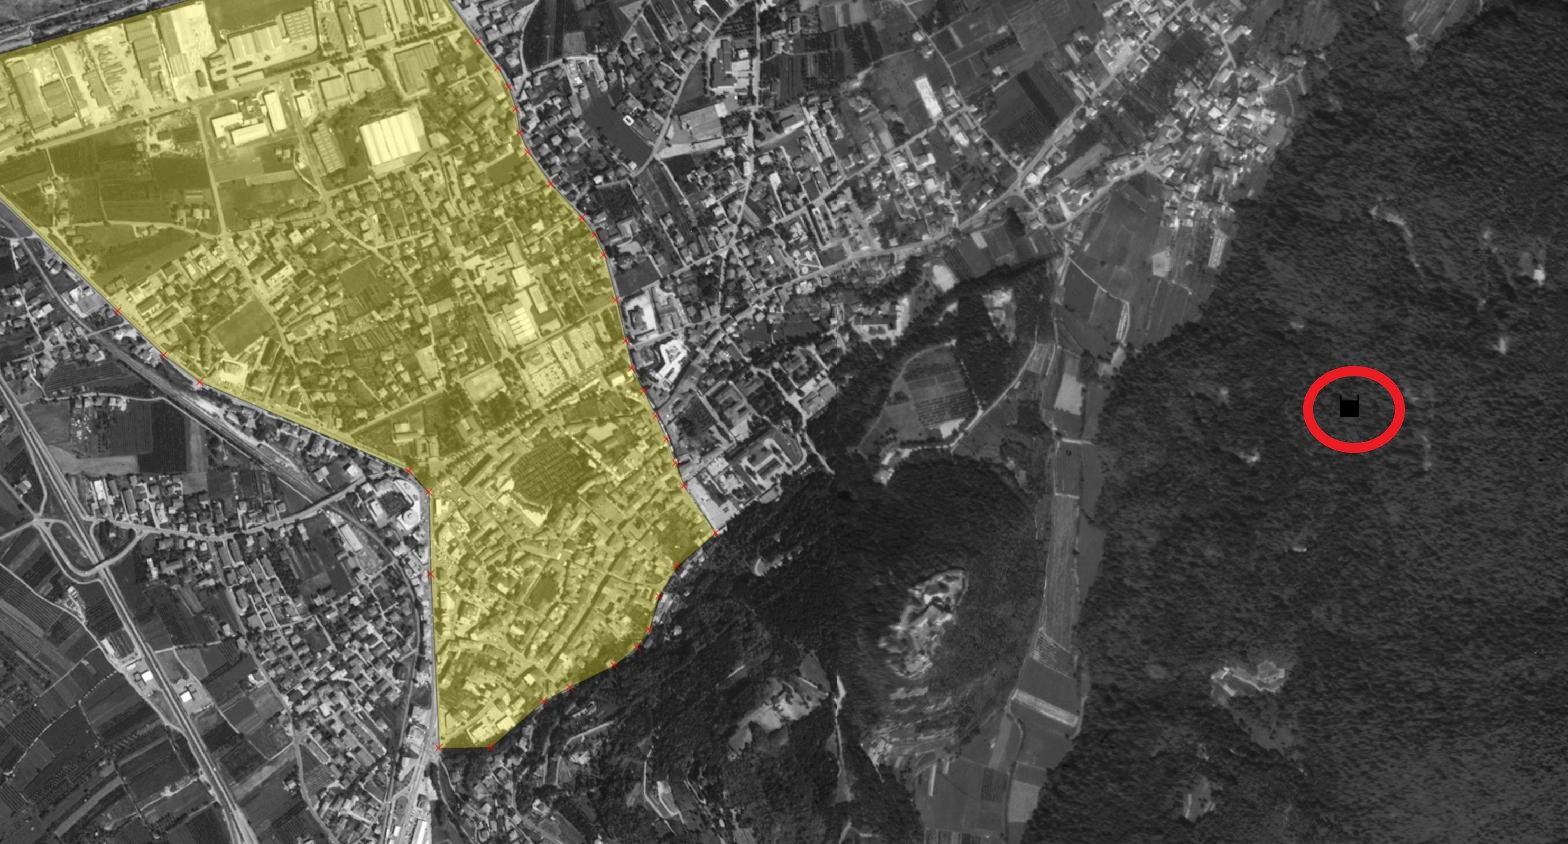
\includegraphics[width=\linewidth]{images/sorgente_01}
       \onslide<2>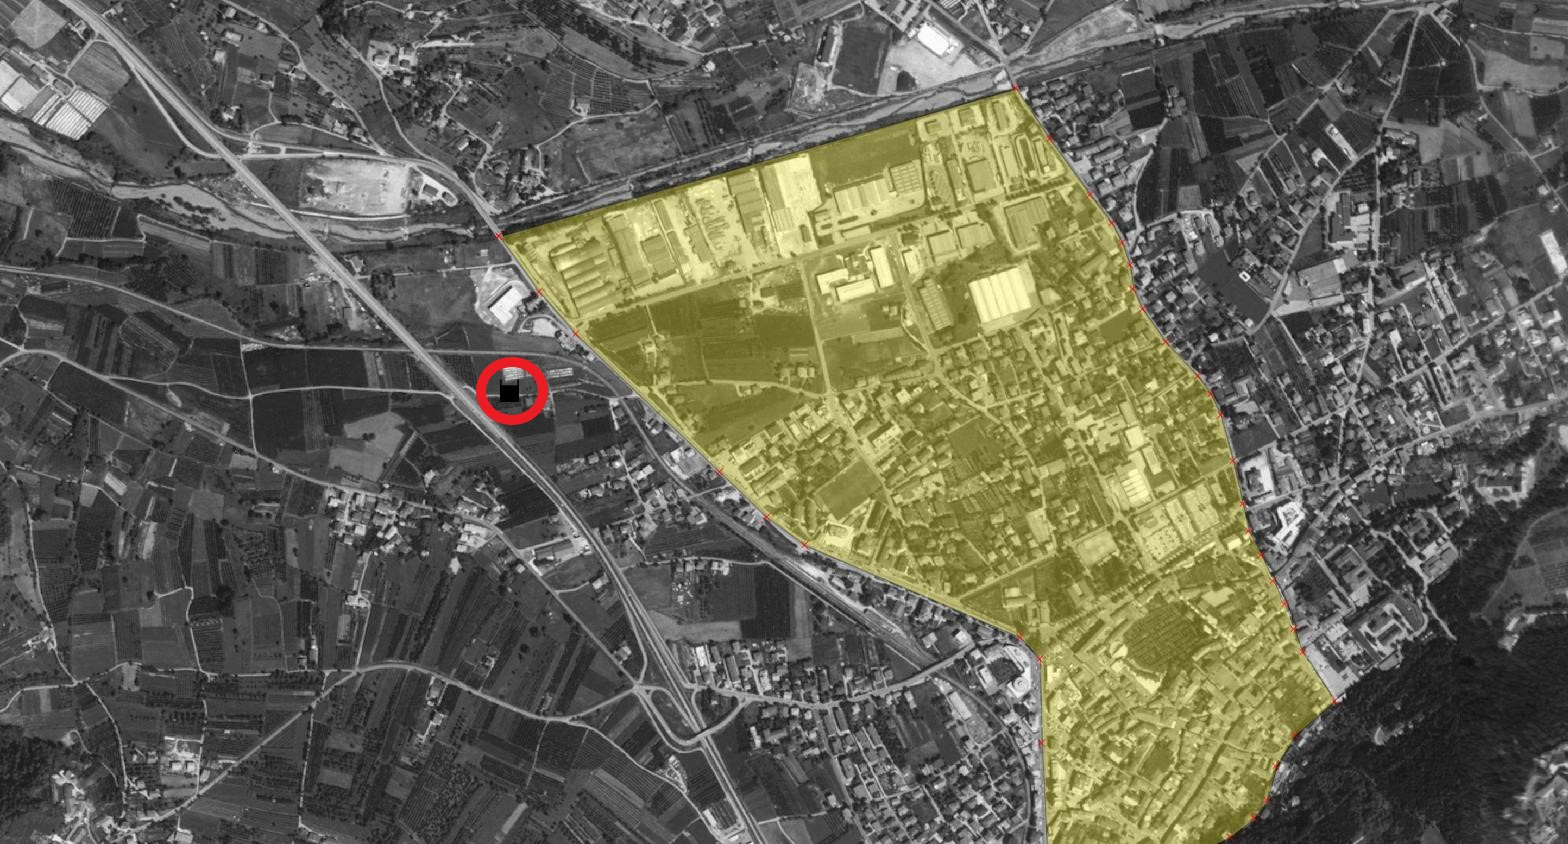
\includegraphics[width=\linewidth]{images/sorgente_02}
      \end{overprint}
     \end{figure}
    \end{column}
%
    \begin{column}{.5\textwidth}
     \begin{itemize}
      \onslide<1>\item sorgente:
      \begin{itemize}
       \item nome: \emph{ciomba 4}
       \item quota: $660.97\,m$
       \item portata: $0.6\,l/_s$
      \end{itemize}
      \onslide<2>\item pozzo:
      \begin{itemize}
       \item ipotesi progettuale
       \item falda freatica
       \item profondità falda: $50\,m$
       \item portata: $1\,l/_s$
       \item utilizzo di una pompa sommersa       
      \end{itemize}
     \end{itemize}
    \end{column}
 \end{columns}
\end{frame}


\section{Progetto dell'acquedotto}
\begin{frame}
 \frametitle{Ipotesi progettuali}
 \begin{itemize}[<+->]
  \item rete a maglia mista
  \item anello principale esterno
  \item anelli secondari interni
  \item rete posta a $1.20\,m$ sotto il piano stradale
  \item impiego di \emph{tubi in acciaio $L235$} con:
  \begin{itemize}[<.->]
   \item protezione esterna con rivestimento bituminoso pesante (secondo la UNI ISO 5256/87)
   \item protezione interna epossidica (conforme al D.M. n. 174 del 06/04/2004)
   \item giunto a bicchiere
  \end{itemize}
 \end{itemize}
\end{frame}

\begin{frame}
 \frametitle{Pompa}
 \begin{columns}
  \begin{column}{.5\textwidth}
   \begin{figure}
    \centering
    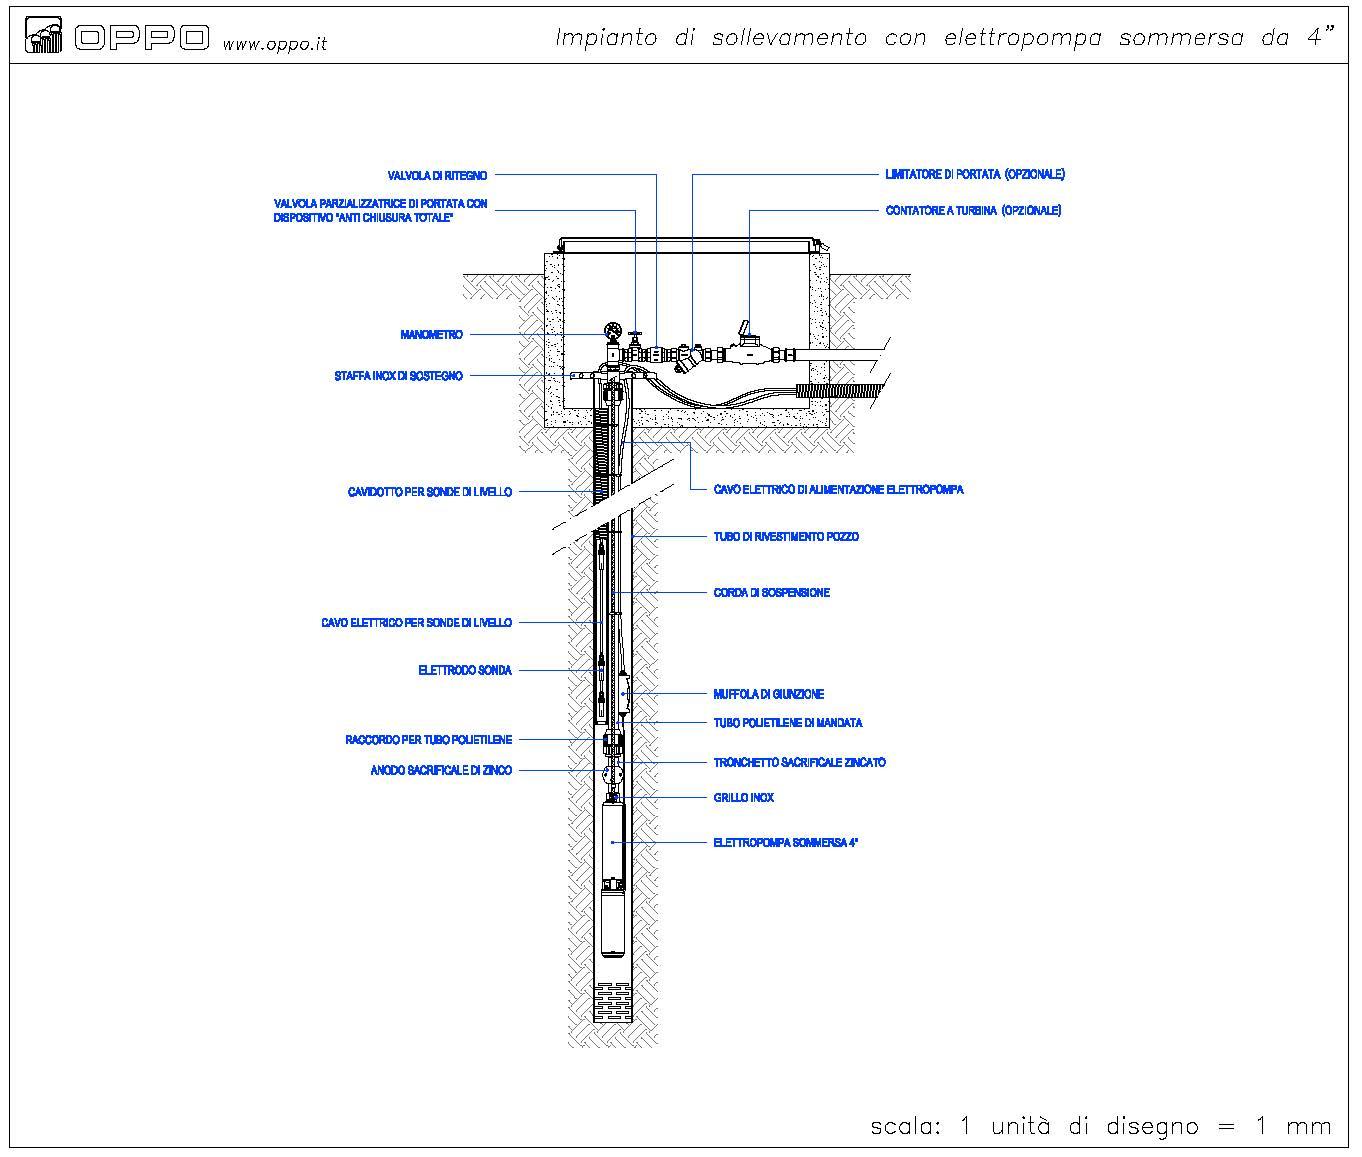
\includegraphics[width=\linewidth]{images/impianto_pompaggio}
    \caption{Fonte: \url{www.oppo.it}}
   \end{figure}
  \end{column}
%
    \begin{column}{.5\textwidth}
     \begin{itemize}
      \item elettropompa sommersa centrifuga \emph{8GS30}
      \item portata fino a $160\,l/_{min}$
      \item potenza: $3\,kW$
      \item alimentazione: $400\,V$
      \item portata: $[58 - 183]\,l/_{min}$
      \item prevalenza: $[123 - 42]\,m$
      \item prezzo: 1145\,\euro
     \end{itemize}

    \end{column}

 \end{columns}

\end{frame}


\begin{frame}
 \frametitle{Creazione della rete su QEpanet}
 
 \begin{columns}
  \begin{column}{.5\textwidth}
   \begin{figure}
    \centering  
    \begin{overprint}
     \onslide<1>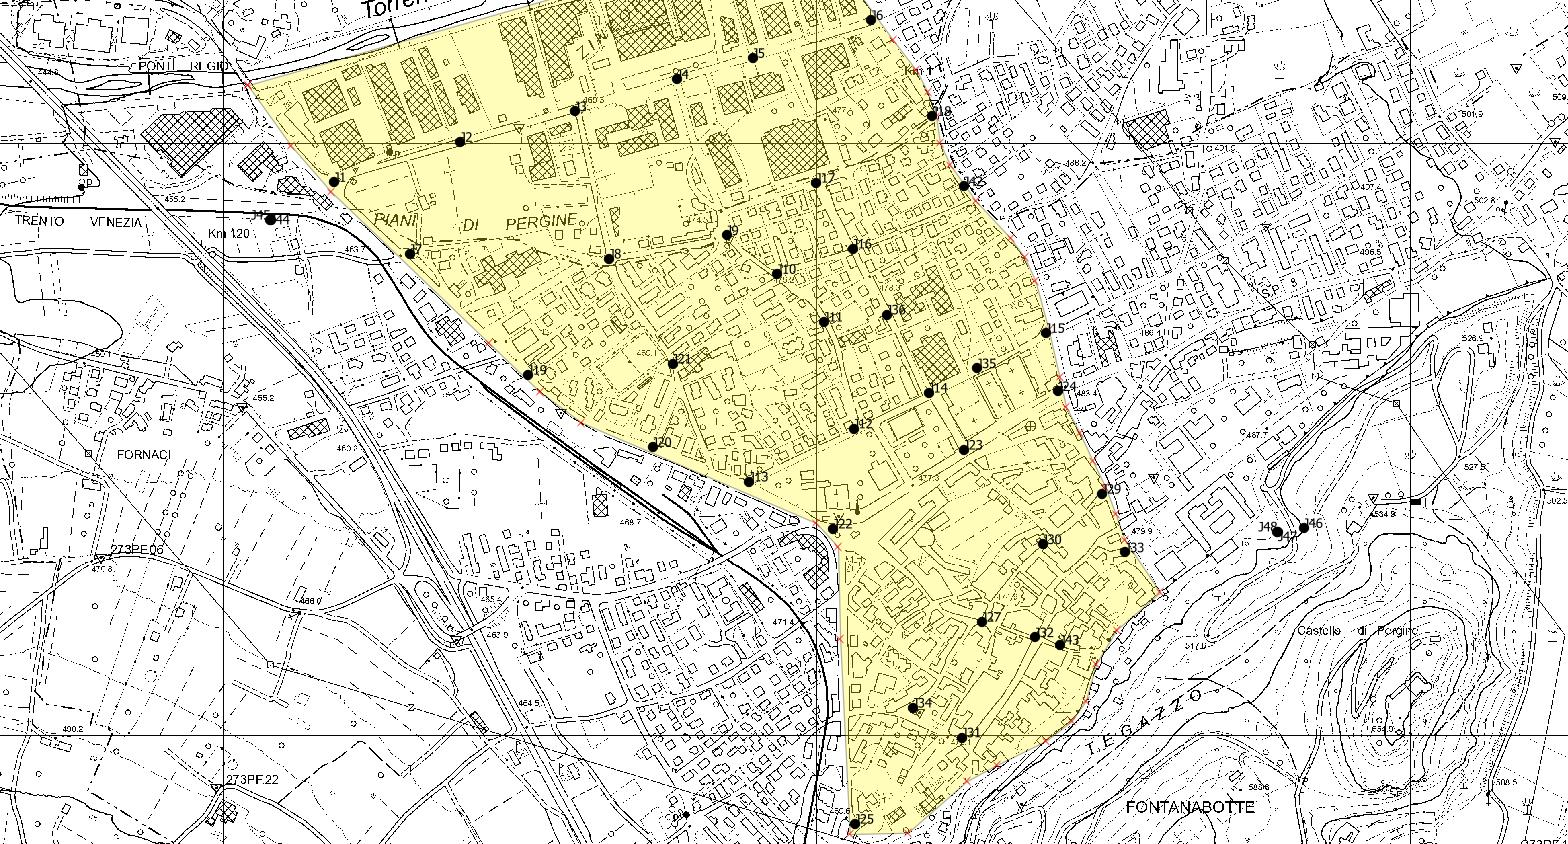
\includegraphics[width=\linewidth]{images/junctions}
     \onslide<2>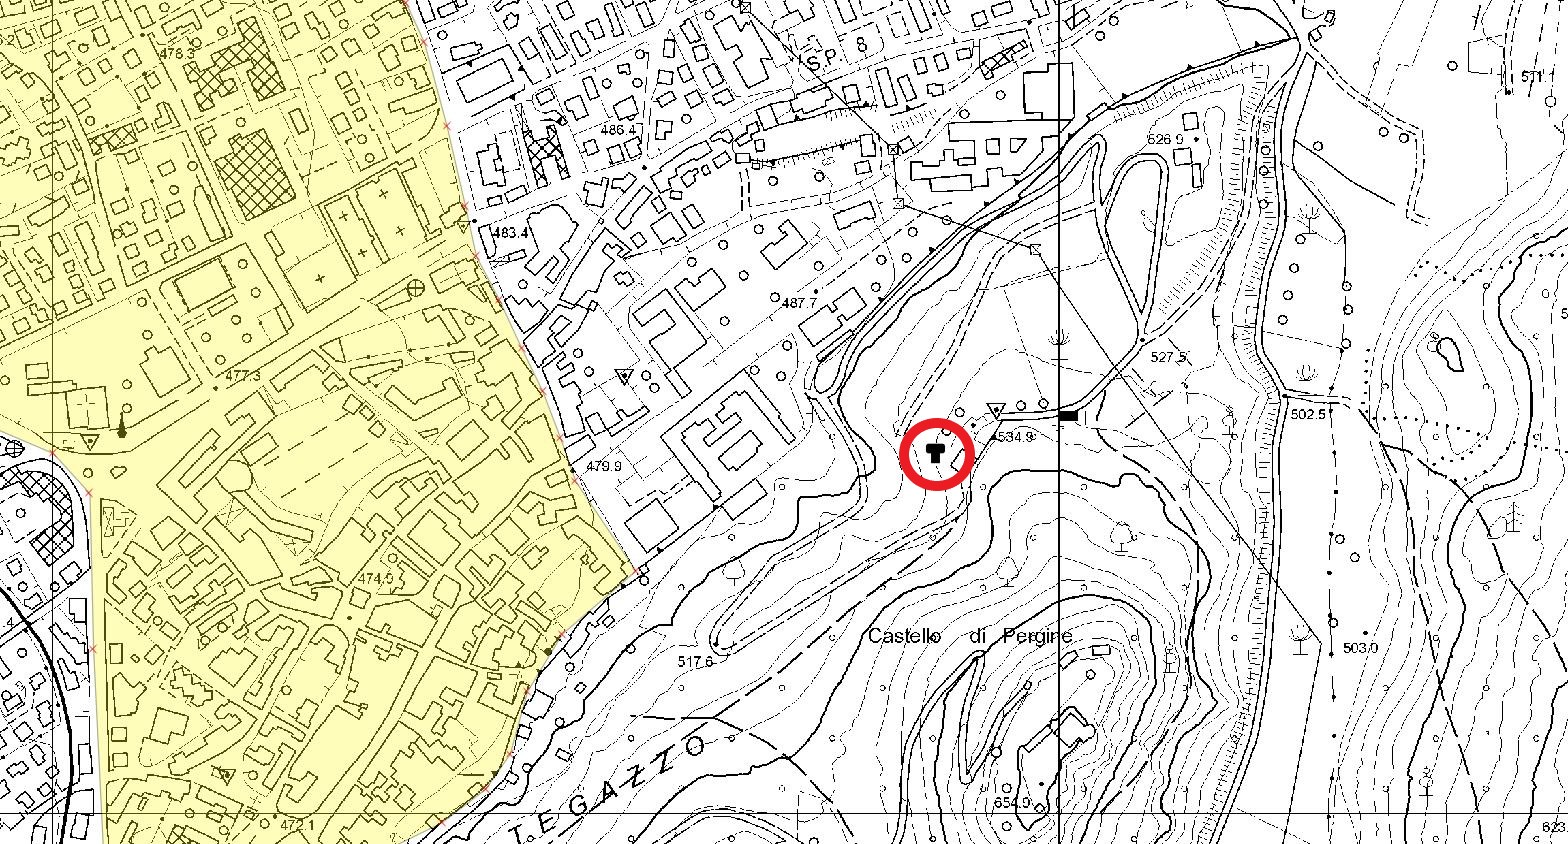
\includegraphics[width=\linewidth]{images/tanks}
     \onslide<3>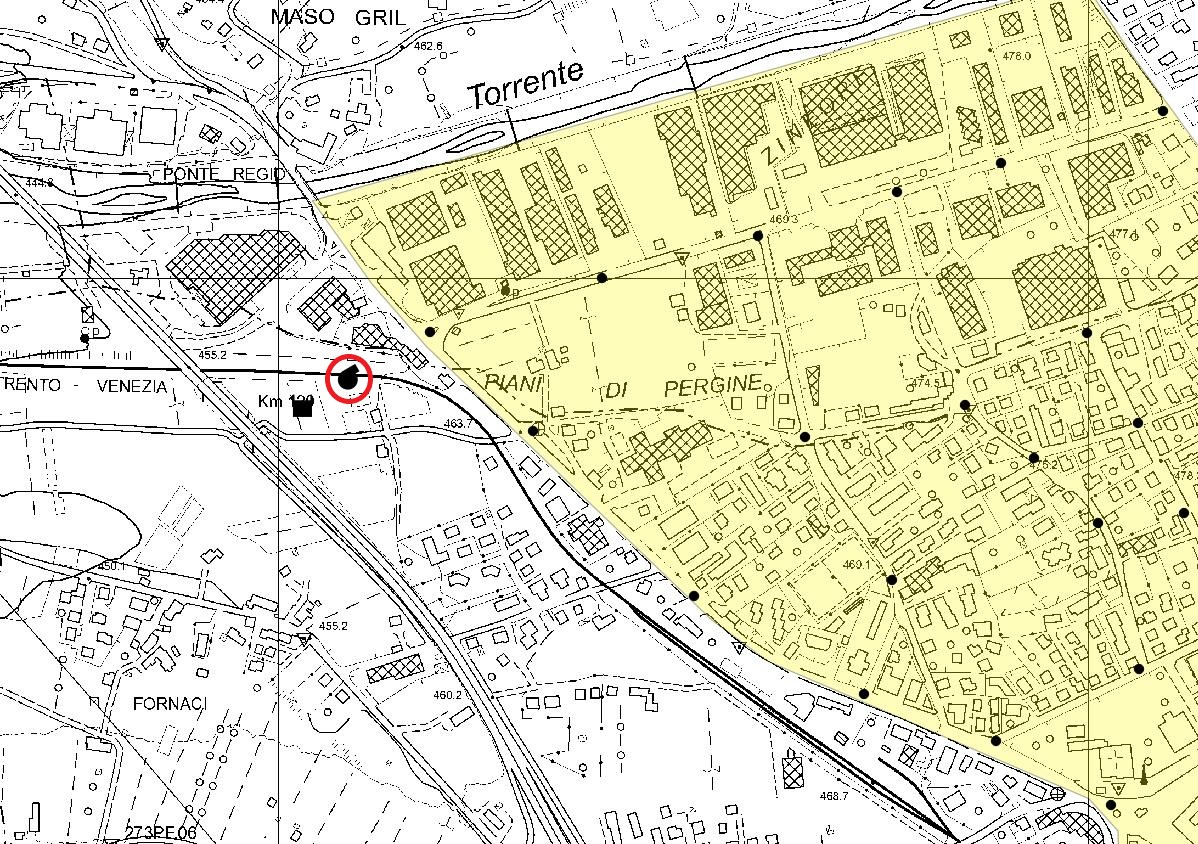
\includegraphics[width=\linewidth]{images/pump}
     \onslide<4>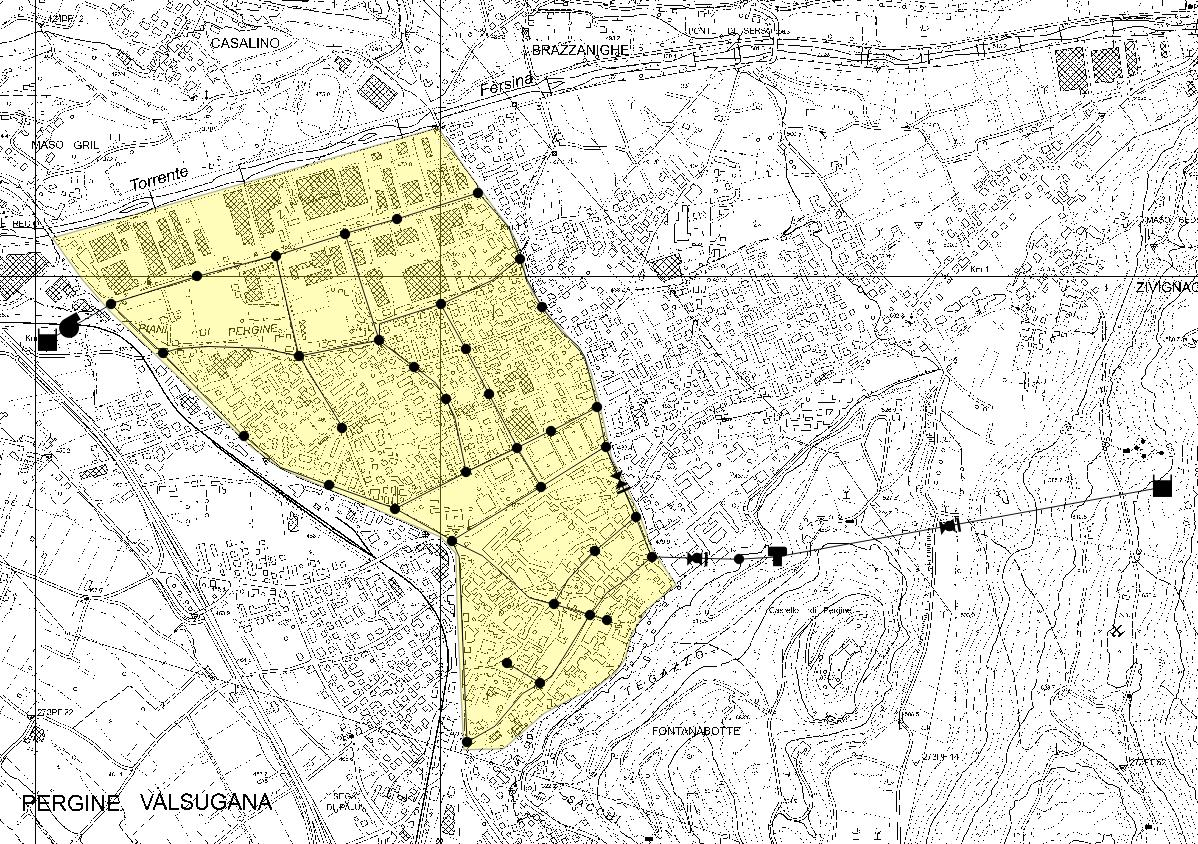
\includegraphics[width=\linewidth]{images/pipes}
    \end{overprint}
   \end{figure}
  \end{column}
  
  \begin{column}{.5\textwidth}
   \begin{itemize}[<+->]
    \onslide<1>\item posizionamento delle $43$ \emph{junctions}, di cui $35$ per la distribuzione idrica
    \onslide<2>\item posizionamento del serbatoio cilindrico di diametro $20\,m$ e altezza $12\,m$ %posto a quota $510.90\,m$
    \onslide<3> \item posizionamento della pompa \emph{8GS30} (da \url{www.oppo.it})
    \onslide<4> \item creazione delle condotte per un totale di $10.12\,km$
   \end{itemize}
  \end{column}
 \end{columns}
\end{frame}
%
%
%
{\nologo
\begin{frame}[allowframebreaks]
 \frametitle{Tabelle per i consumi idrici giornalieri}
 \begin{columns}
  \begin{column}{.45\textwidth}
   \begin{figure}
    \centering
    \subfloat{}{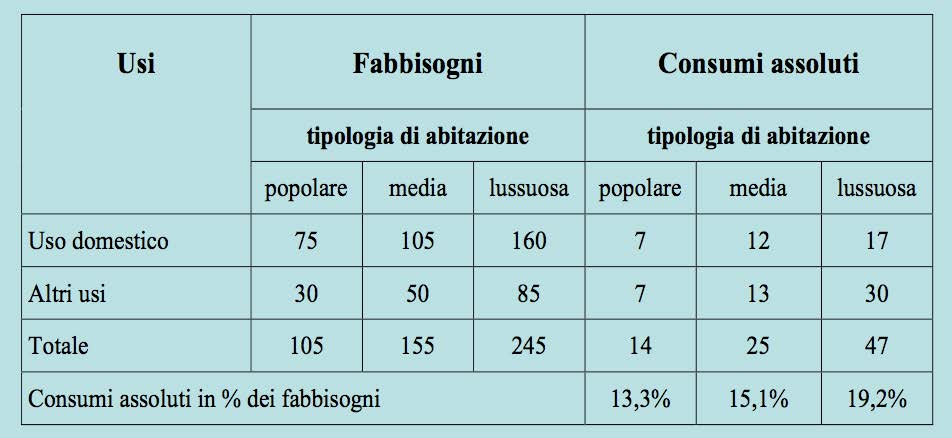
\includegraphics[height=.225\pdfpageheight]{images/tabella_fabbisogni_domestici}}\\[1.5ex]
    \subfloat{}{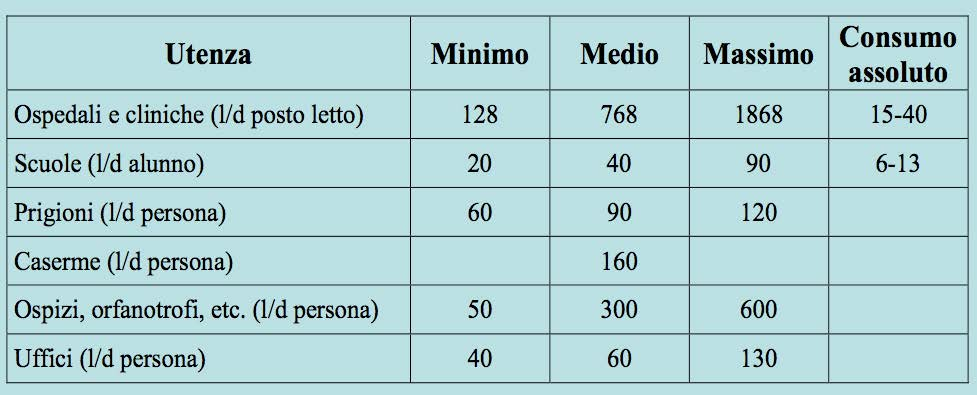
\includegraphics[height=.22\pdfpageheight]{images/tabella_fabbisogni_pubblici}}\\[1.5ex]
    \subfloat{}{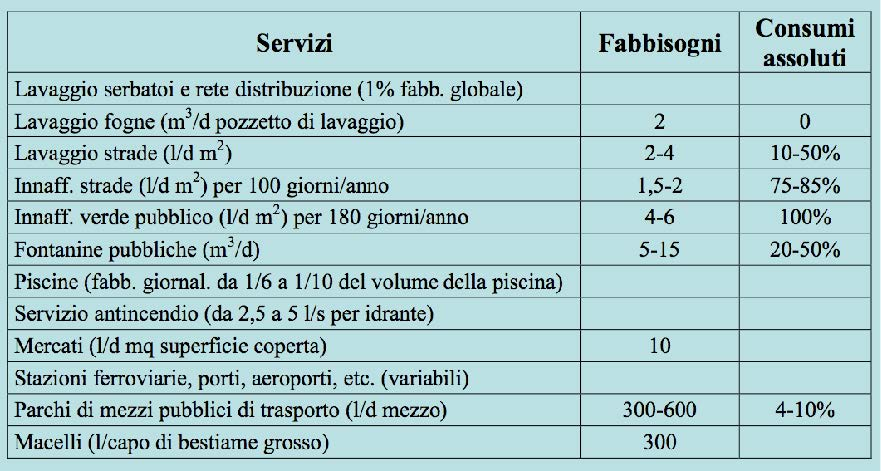
\includegraphics[height=.25\pdfpageheight]{images/tabella_fabbisogni_servizi}}
   \end{figure}
  \end{column}
%
  \begin{column}{0.55\textwidth}
   \begin{itemize}
		\item zona residenziale:
    \begin{itemize}
     \item $105\,l/_{gg\,ab}$ per zone periferiche
     \item $155\,l/_{gg\,ab}$ in centro storico e zone limitrofe
     \item densità di $0.0125\,ab/m^2$ (fonte \href{http://cartografia.comune.pergine.tn.it/PRG_Vigente/documenti/main.html}{\emph{PRG Pergine Valsugana}})
    \end{itemize}
    \item poli scolastici: 
    \begin{itemize}
     \item $50\,l/_{gg\,alunno}$
     \item scuola primaria: 14 classi (fonte \href{http://www.icpergine1.it/}{\emph{Istituto Comprensivo di Pergine 1}}), da $20$ alunni (ipotesi) per un totale di 280 studenti
     \item scuola secondaria: 16 classi da $20$ alunni per un totale di $320$ studenti
    \end{itemize}
   \end{itemize}
  \end{column}
 \end{columns}
\framebreak
%
\begin{columns}
  \begin{column}{.45\textwidth}
   \begin{figure}
    \centering
    \subfloat{}{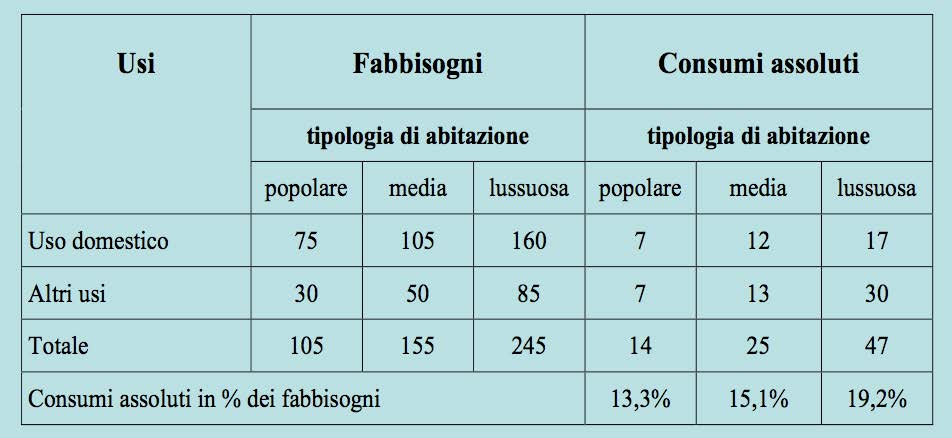
\includegraphics[height=.225\pdfpageheight]{images/tabella_fabbisogni_domestici}}\\[1.5ex]
    \subfloat{}{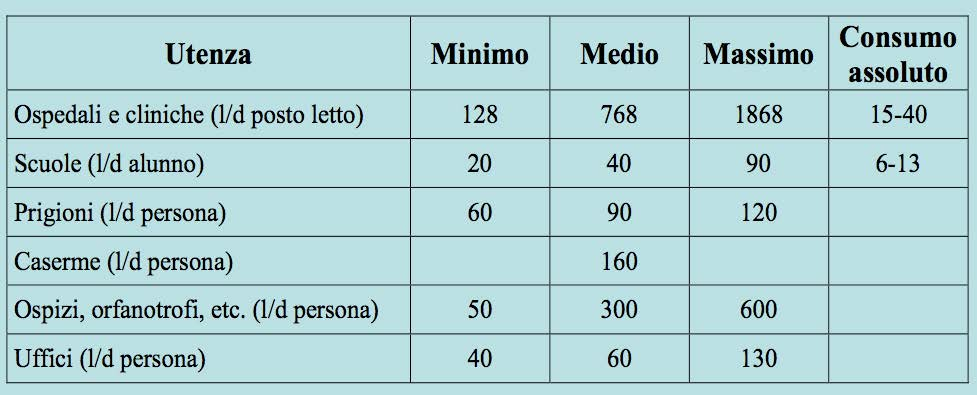
\includegraphics[height=.22\pdfpageheight]{images/tabella_fabbisogni_pubblici}}\\[1.5ex]
    \subfloat{}{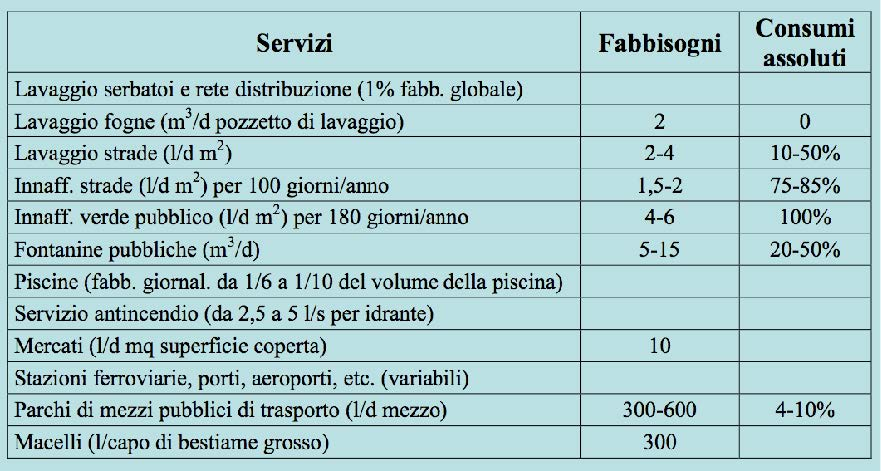
\includegraphics[height=.25\pdfpageheight]{images/tabella_fabbisogni_servizi}}
   \end{figure}
  \end{column}
%
  \begin{column}{0.55\textwidth}
   \begin{itemize}
    \item zona industriale:
    \begin{itemize}
     \item $100\,l/_{gg\,addetto}$
     \item numero di addetti da \url{https://it.kompass.com/}
    \end{itemize}
    \item caserma dei vigili del fuoco: 
    \begin{itemize}
     \item consumo di $160\,l/_{gg\,persona}$
     \item $89$ persone (fonte \url{https://www.vvf-perginevalsugana.it/chi-siamo})
    \end{itemize}
    \item zona turistica:
    \begin{itemize}
     \item zona turistica 1: consumo di $30\,l/_{gg\,m^2}$
     \item zona turistica 2:
     \begin{itemize}
      \item consumo di $30\,l/_{gg\,pasto}$
      \item ipotesi di $80\,pasti/_{gg}$
     \end{itemize}
    \end{itemize}
   \end{itemize}
  \end{column}
 \end{columns}
\framebreak
%
\begin{columns}
  \begin{column}{.45\textwidth}
   \begin{figure}
    \centering
    \subfloat{}{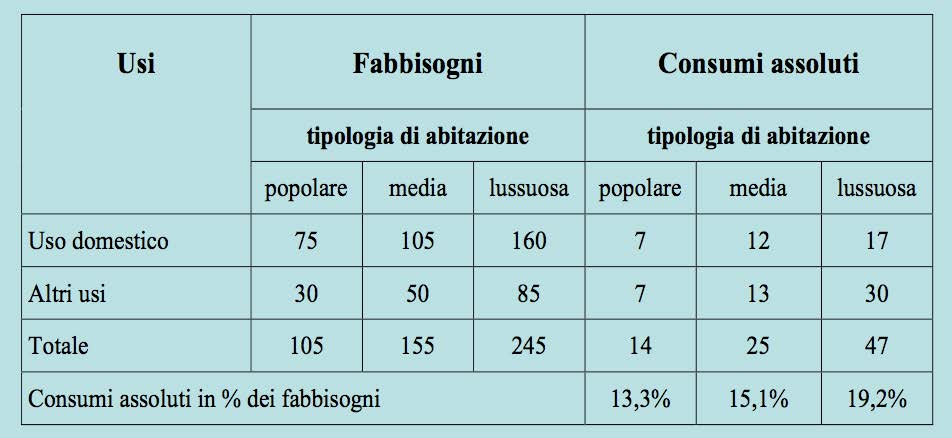
\includegraphics[height=.225\pdfpageheight]{images/tabella_fabbisogni_domestici}}\\[1.5ex]
    \subfloat{}{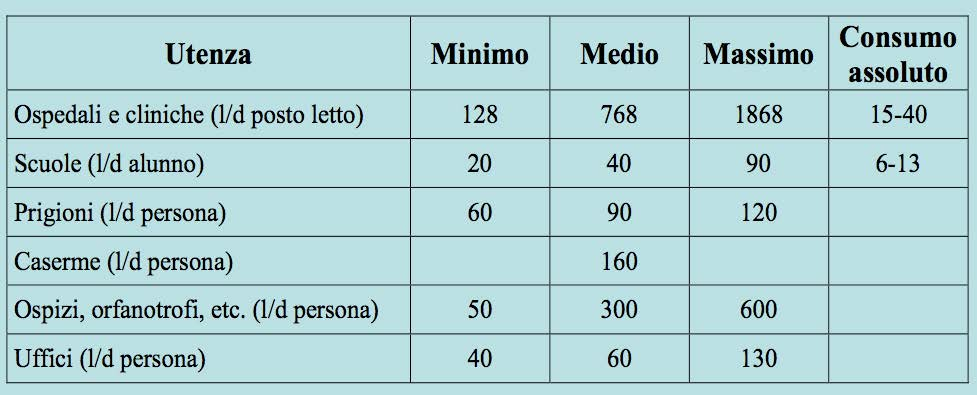
\includegraphics[height=.22\pdfpageheight]{images/tabella_fabbisogni_pubblici}}\\[1.5ex]
    \subfloat{}{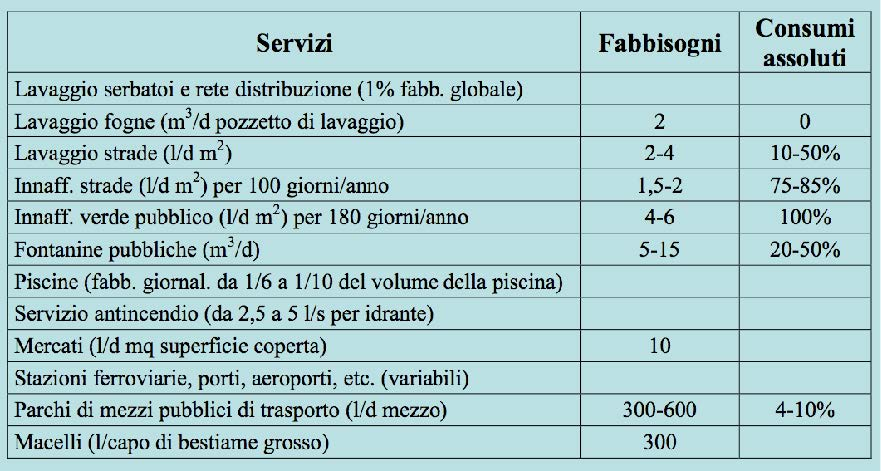
\includegraphics[height=.25\pdfpageheight]{images/tabella_fabbisogni_servizi}}
   \end{figure}
  \end{column}
%
  \begin{column}{0.55\textwidth}
   \begin{itemize}
    \item piscina comunale:
    \begin{itemize}
     \item fabbisogno di $1/_6$ del volume di acqua totale
     \item ipotesi di $3$ piscine per un totale di $1400\,m^3$
     \item consumo giornaliero di $230\,l$
    \end{itemize}
    \item aree verdi: consumo di $5\,l/_{gg}$ per irrigazione
   \end{itemize}
  \end{column}
 \end{columns}
\end{frame}
}
%
%
%
\begin{frame}
 \frametitle{Calcolo del fabbisogno idrico giornaliero}
	Definizione dei nodi di emungimento per ogni area e della portata ai nodi necessaria, attraverso i dati ricavati in precedenza.	
   \begin{figure}
    \centering
    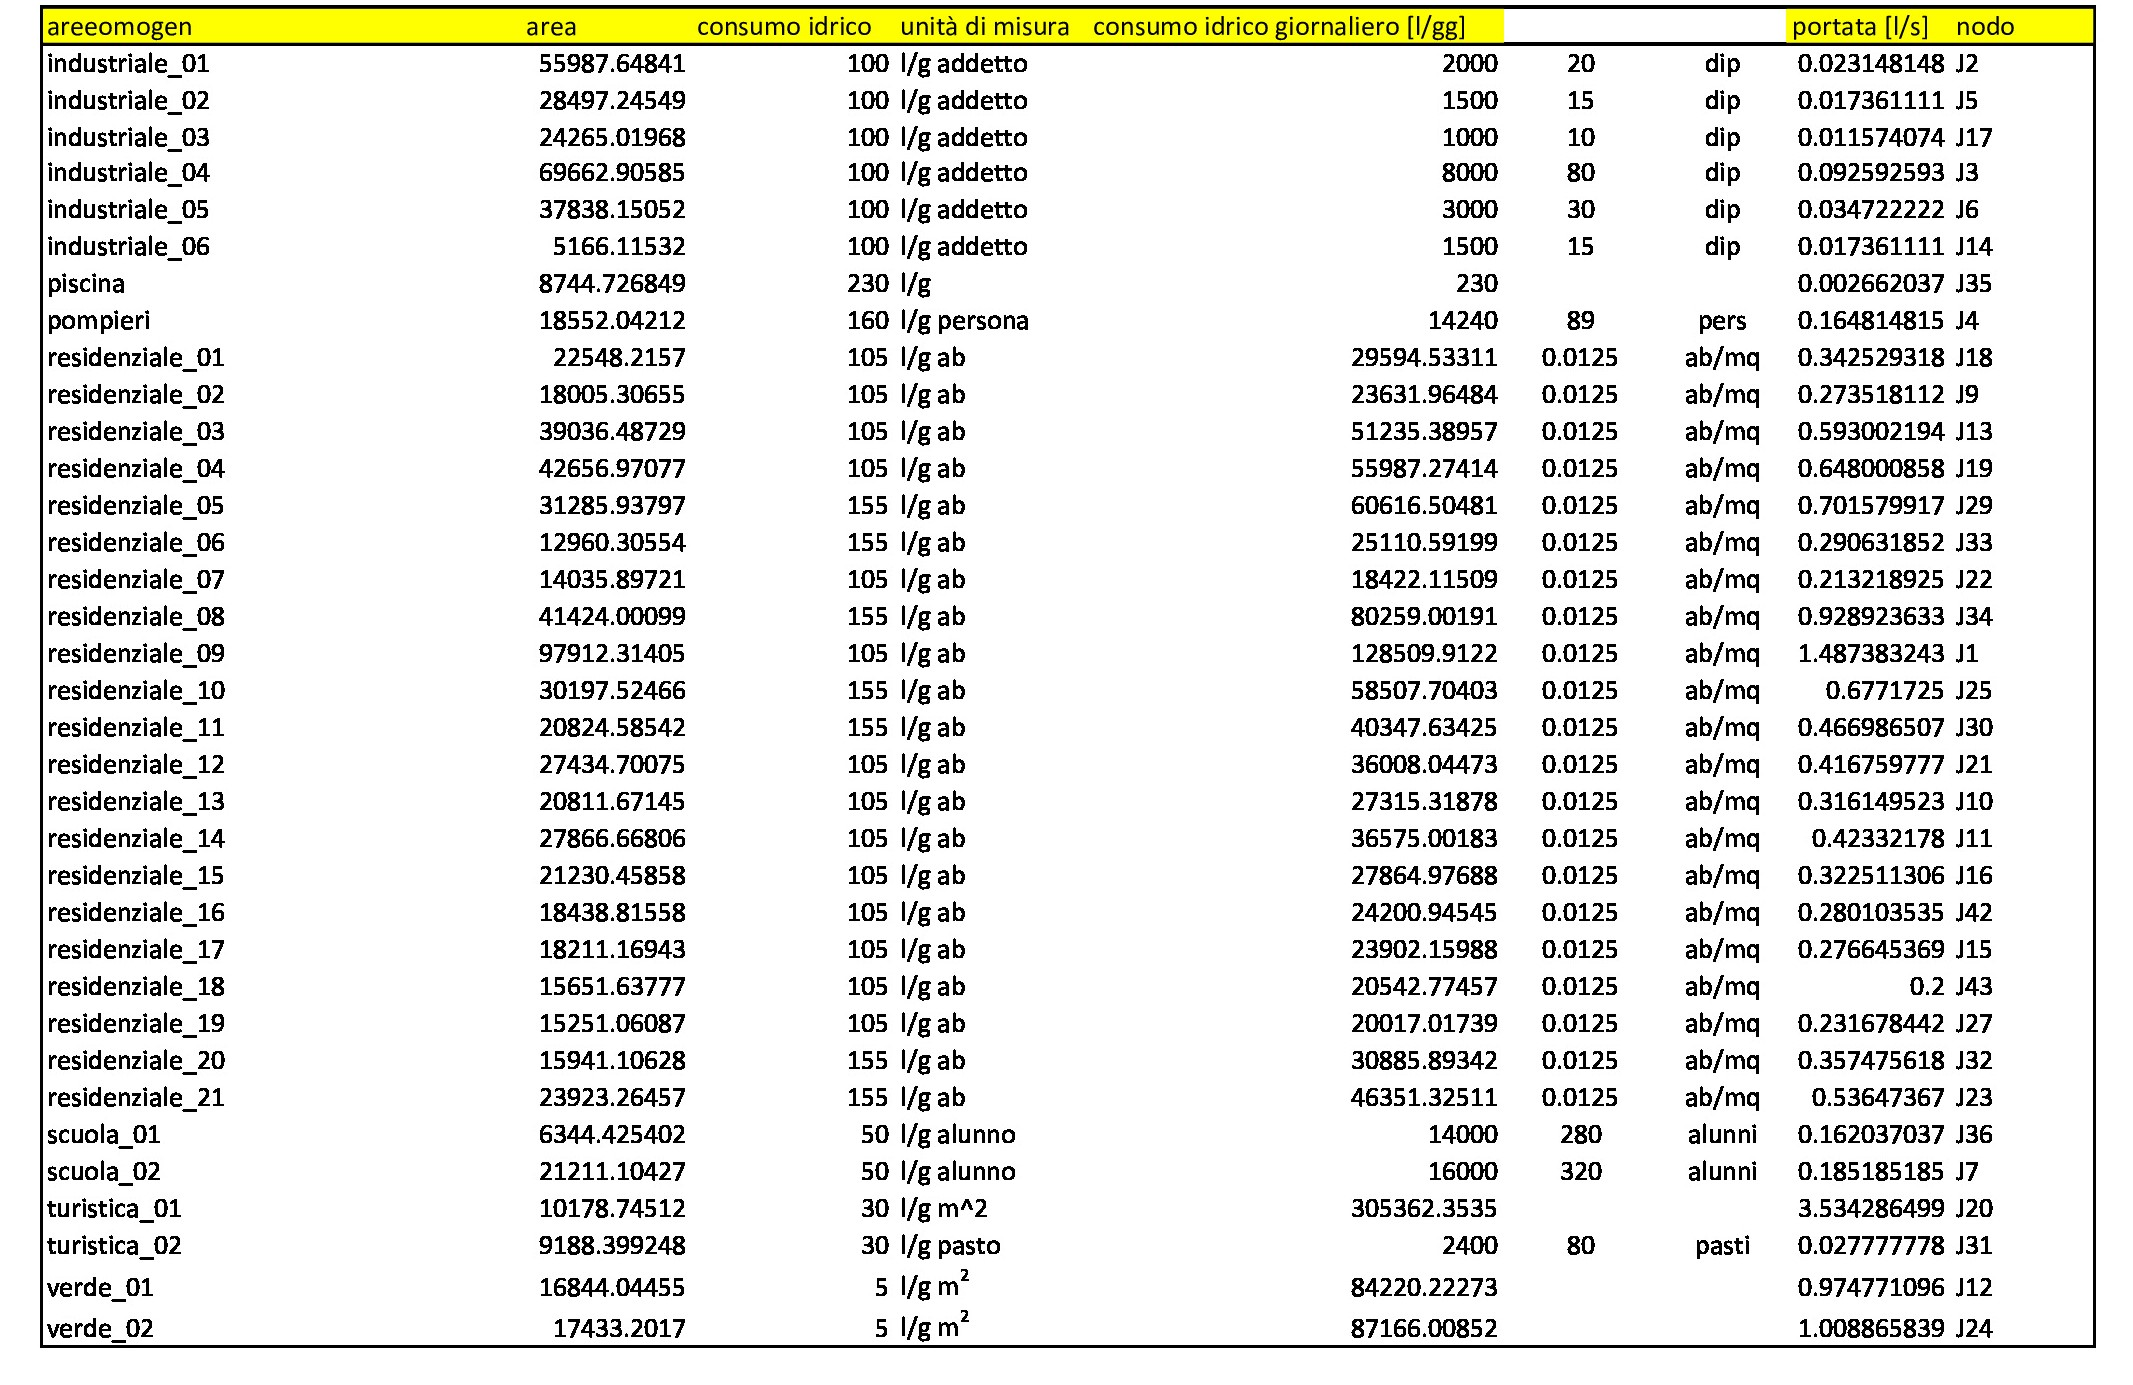
\includegraphics[width=.7\linewidth]{images/calcolo_consumo_idrico}
   \end{figure}
\end{frame}
%
\begin{frame}
 \frametitle{Calcolo del fabbisogno idrico giornaliero}
 \framesubtitle{Coefficiente di punta giornaliero}
 Calcolo del coefficiente di punta giornaliero, pari a
 \[
  K_g = 1.15
 \]

   \begin{figure}
    \centering
    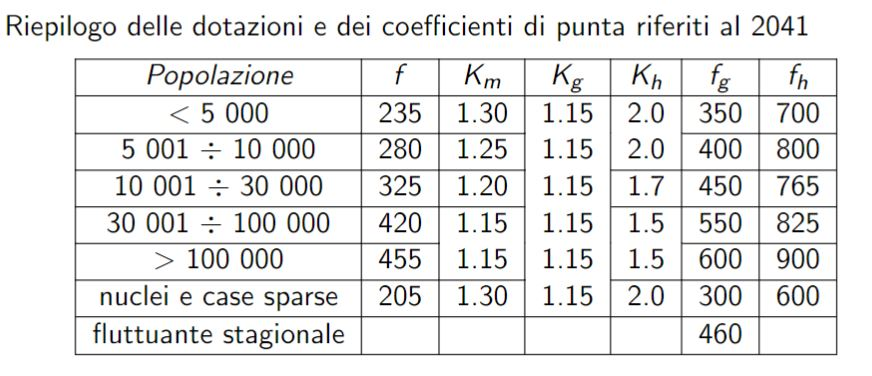
\includegraphics[width=.7\linewidth]{images/coefficienti_punta}
   \end{figure}
\end{frame}
%
\begin{frame}
 \frametitle{Calcolo del fabbisogno idrico giornaliero}
 \framesubtitle{Fabbisogno idrico finale}
Il fabbisogno giornaliero totale è di 
\[
 1617480.369\,\dfrac{l}{gg} = 18.72\,\dfrac{l}{s}
\]

   \begin{figure}
    \centering
    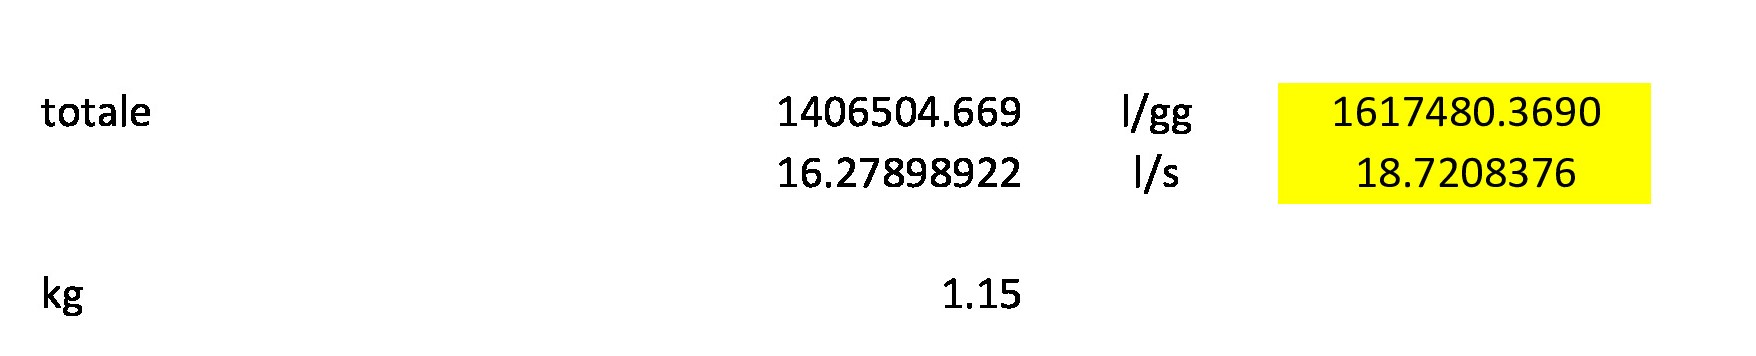
\includegraphics[width=.7\linewidth]{images/fabbisogno_totale}
   \end{figure}
\end{frame}
%
%
%
\begin{frame}
	\frametitle{Creazione dei pattern}
	\begin{columns}
	 \begin{column}{.5\textwidth}
	  \begin{figure}
	   \centering
	   \begin{overprint}
	   \onslide<1>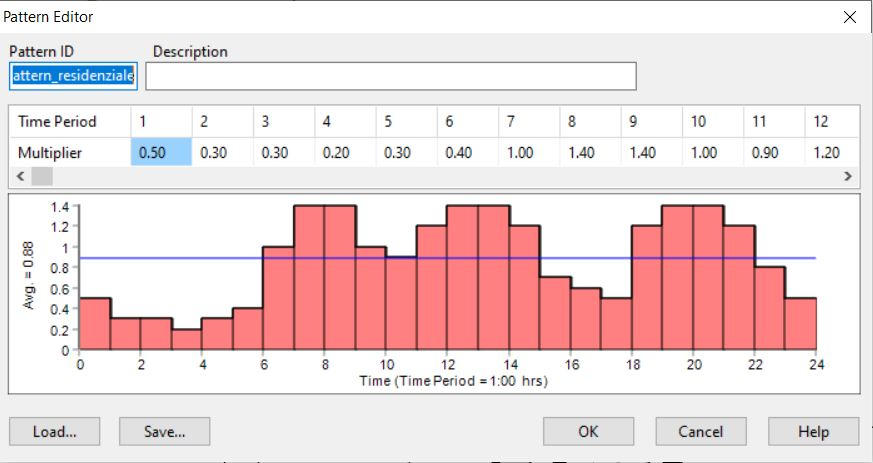
\includegraphics[width=\linewidth]{images/pattern_residenziale}
	   \onslide<2>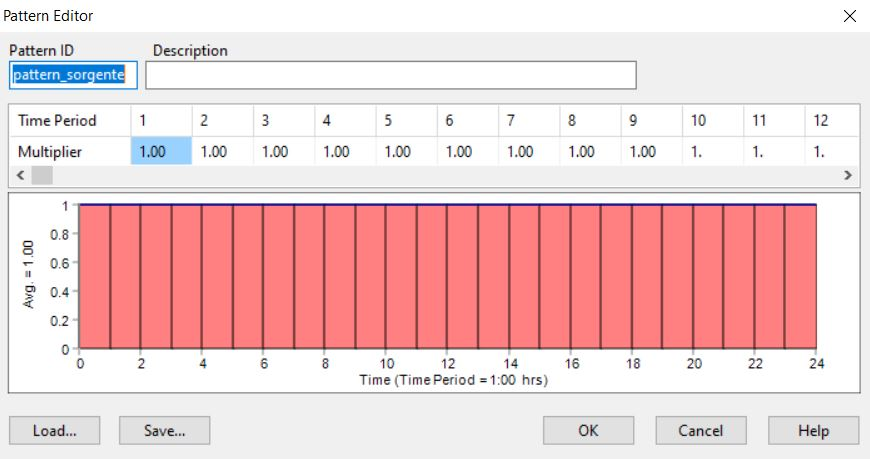
\includegraphics[width=\linewidth]{images/pattern_sorgente}
	   \onslide<3>
	   \begin{center}
	    \subfloat{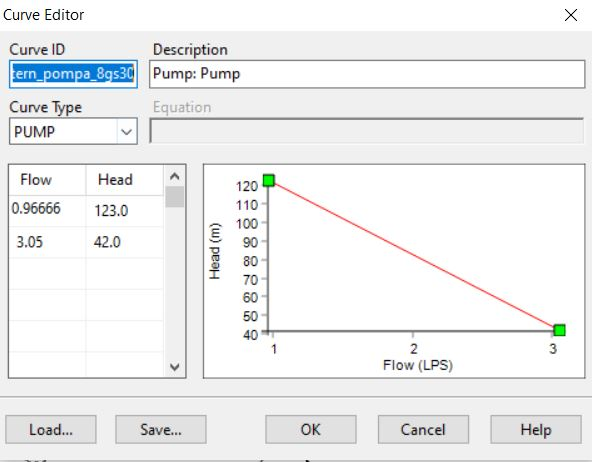
\includegraphics[height=.4\paperheight]{images/curva_pompa}}\\
	   \end{center}
	   \subfloat{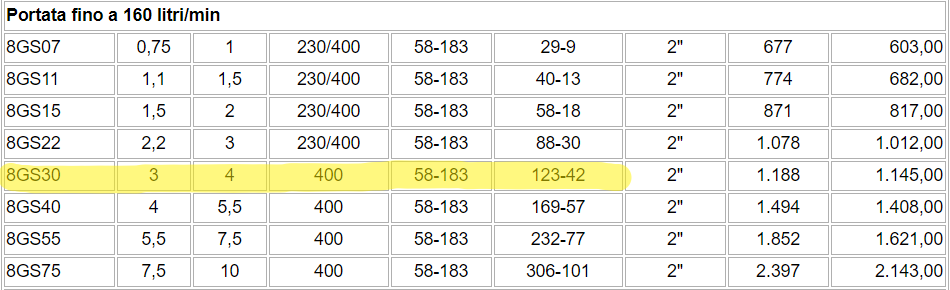
\includegraphics[width=\linewidth]{images/dati_pompa}}
	  \end{overprint}
	  \end{figure}
	 \end{column}
%
	\begin{column}{.5\textwidth}
		\begin{itemize}[<+->]
		 \onslide<1>\item creazione dei pattern per ogni area omogenea
		 \onslide<2>\item creazione di un pattern per sorgente e pozzo
		 \onslide<3>\item definizione della curva della pompa (fonte \href{https://www.oppo.it/materiali/pompe/elettr_pompa-sommerse-4.html}{oppo.it})
		\end{itemize}
	\end{column}
	\end{columns}
\end{frame}
%
\begin{frame}
	\frametitle{Dimensionamento delle tubazioni}
	 \begin{table}
	 \caption{Da \href{https://www.oppo.it/materiali/tubi_raccordi/acciao-bitumati-sal-tubi.html}{oppo.it}}
	  \begin{tabular}{lccr}
	  \toprule
	   posizione &$D_N\,[mm]$ &$\Phi_{ext}\,[mm]$ &$s\,[mm]$\\
	   \midrule
	   anello esterno &$100$ & $114.3$ &$3.2$\\
	   anelli interni &$80$ & $88.9$ &$2.9$\\
	   adduzione pozzo &$100$ & $114.3$ &$3.2$\\
	   \begin{tabular}{@{}l@{}}adduzione\\ sorgente-serbatoio\end{tabular} &$250$ & $273$ &$5.6$\\
	   \begin{tabular}{@{}l@{}}adduzione\\ dopo serbatoio\end{tabular} &$125$ & $139.7$ &$3.6$\\
	   \bottomrule
	  \end{tabular}
	 \end{table}
\end{frame}

%
%
%
\section{Analisi della rete}
\begin{frame}
 \frametitle{Analisi su Epanet}{\allowbreak}
 \begin{columns}
	 \begin{column}{.5\textwidth}
	  \begin{figure}
	   \centering
	   \begin{overprint}
	   \onslide<1>\subfloat{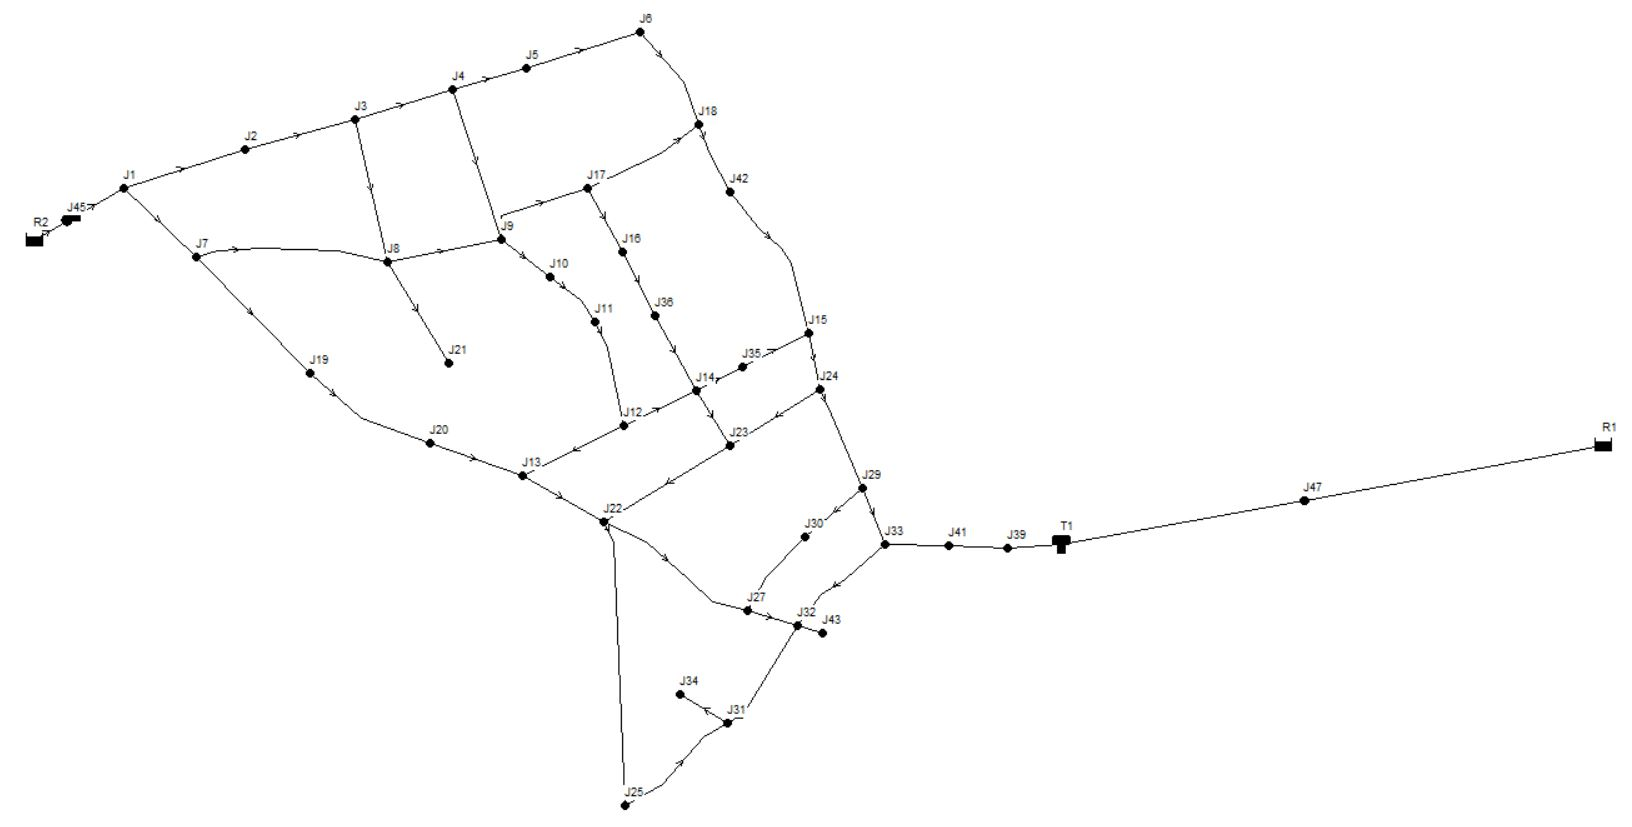
\includegraphics[width=\linewidth]{images/network_without_valves}}\\
	   \subfloat{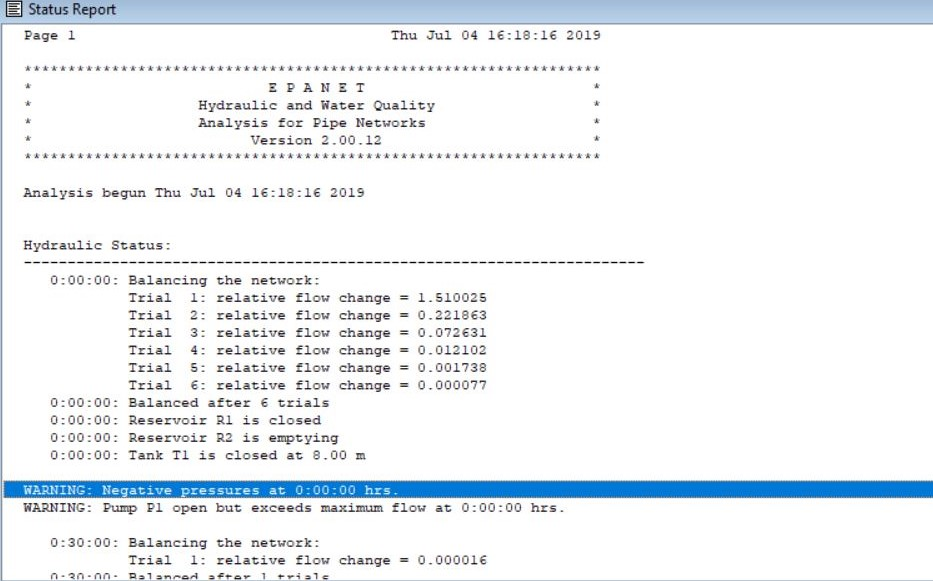
\includegraphics[width=\linewidth]{images/warning_network_without_valves}}
	   \onslide<2>\subfloat{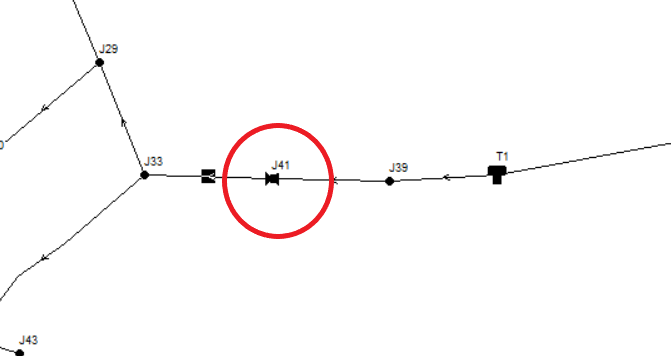
\includegraphics[width=\linewidth]{images/valve_v1}}\vspace{.5mm}
	   \begin{center}
	   \subfloat{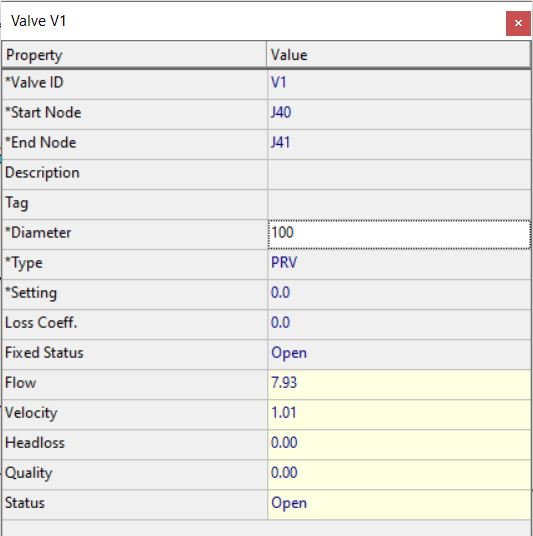
\includegraphics[height=.35\pdfpageheight]{images/v1_properties}}
	   \end{center}
%
		\onslide<3>
		\begin{minipage}[c][.8\textheight][c]{\linewidth}
			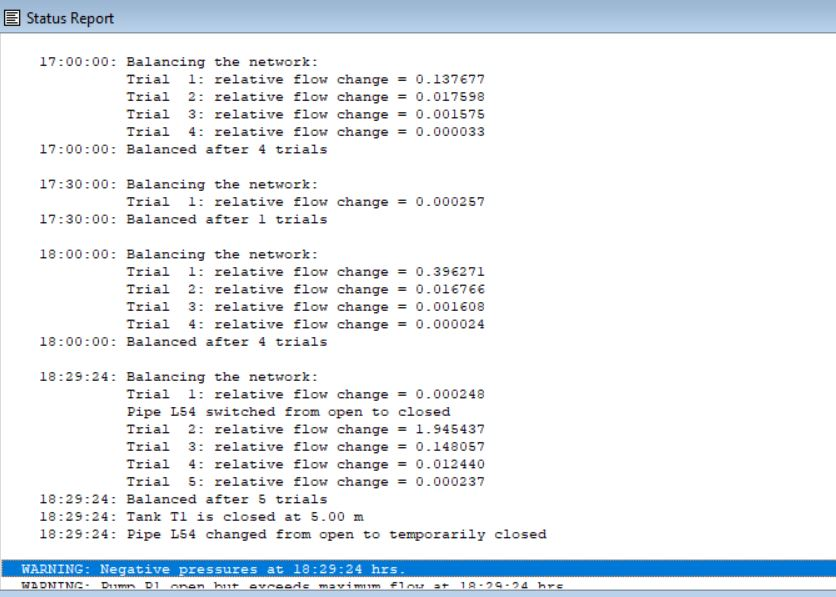
\includegraphics[width=\linewidth]{images/v1_analysis}
		\end{minipage}
%
		\onslide<4>
		\begin{minipage}[c][.8\textheight][c]{\linewidth}
			\centering
			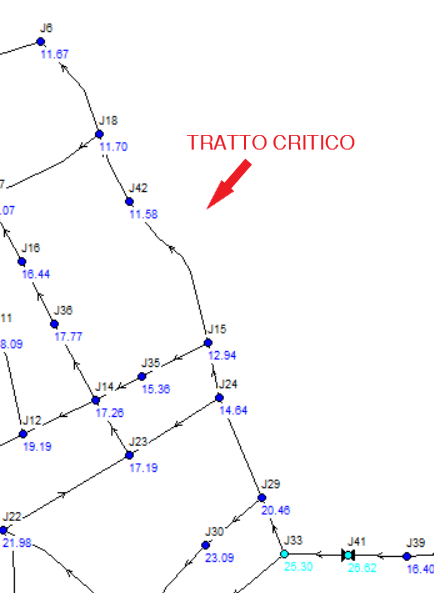
\includegraphics[height=.7\pdfpageheight]{images/tratto_critico}
		\end{minipage}
	  \end{overprint}
	  \end{figure}
	 \end{column}
%
	\begin{column}{.5\textwidth}
		\begin{itemize}[<+->]
		 \onslide<1>\item così com'è, la rete risulta \textbf{non verificata} (pressioni negative)
		 \onslide<2>\item inserimento \emph{valvola PRV} di $D_N = 100\,mm$ dopo il serbatoio
		 \onslide<3>\item anche se migliorata, la rete non è verificata
		 \onslide<4>\item si può notare che è presente un tratto con criticità maggiore degli altri 
		\end{itemize}
	\end{column}
 \end{columns}
\end{frame}
%

%
\begin{frame}
\frametitle{Analisi su Epanet}
	\begin{columns}
	 \begin{column}{.5\textwidth}
	  \begin{figure}
	   \centering
	   \begin{overprint}
	   \onslide<1>\subfloat{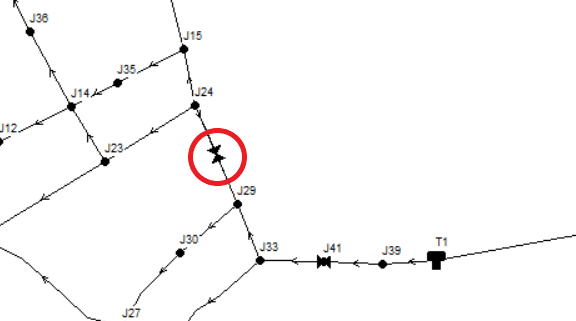
\includegraphics[width=\linewidth]{images/valve_v2}}\vspace{.5mm}
	   \begin{center}
	   \subfloat{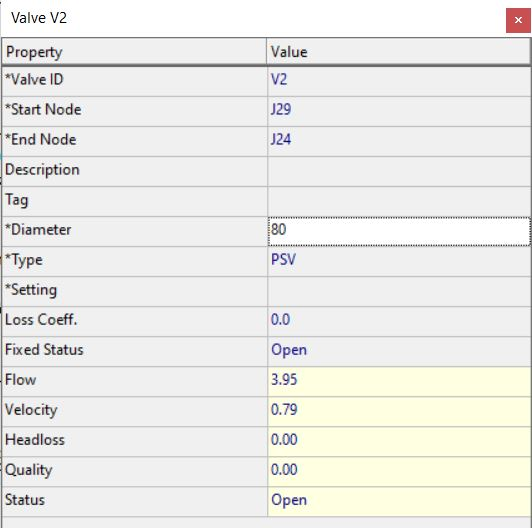
\includegraphics[height=.35\pdfpageheight]{images/v2_properties}}
	   \end{center}
%
	   \onslide<2>\subfloat{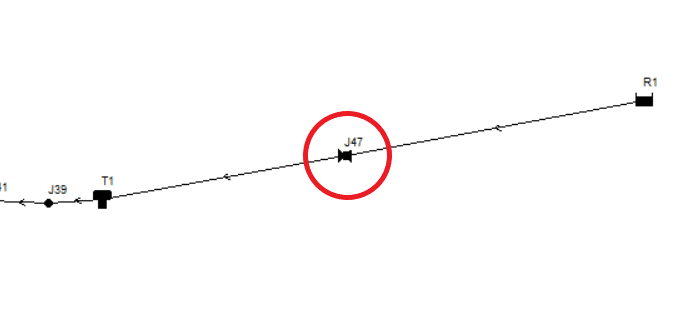
\includegraphics[width=\linewidth]{images/valve_v3}}\vspace{.5mm}
	   \begin{center}
	   \subfloat{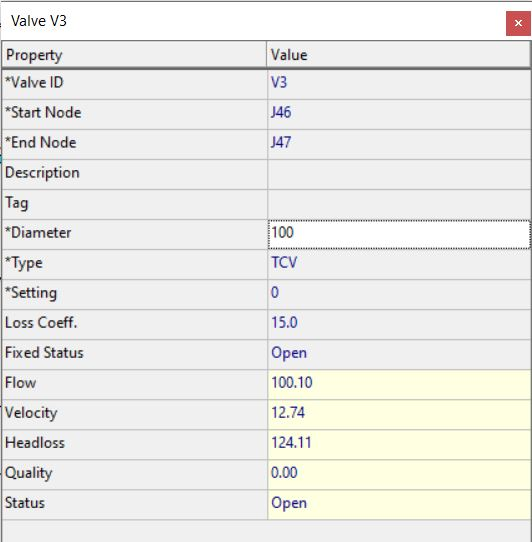
\includegraphics[height=.35\pdfpageheight]{images/v3_properties}}
	   \end{center}
	  \end{overprint}
	  \end{figure}
	 \end{column}
%
	\begin{column}{.5\textwidth}
		\begin{itemize}[<+->]
		\onslide<1>\item inserimento di una \emph{PSV} di $D_N = 80\,mm$ per aumentare il carico nel tratto critico ed evitare la cavitazione	
		 \onslide<2>\item inserimento di una \emph{valvola TCV} di $D_N = 100\,mm$ sulla condotta di adduzione della sorgente per ridurre la velocità dell'acqua
		\end{itemize}
	\end{column}
 \end{columns}
\end{frame}
%
{\nologo
\begin{frame}
\frametitle{Analisi su Epanet}
	\begin{columns}
	 \begin{column}{.5\textwidth}
	  \begin{figure}
	   \centering
	   \begin{overprint}
	   \onslide<1>\subfloat{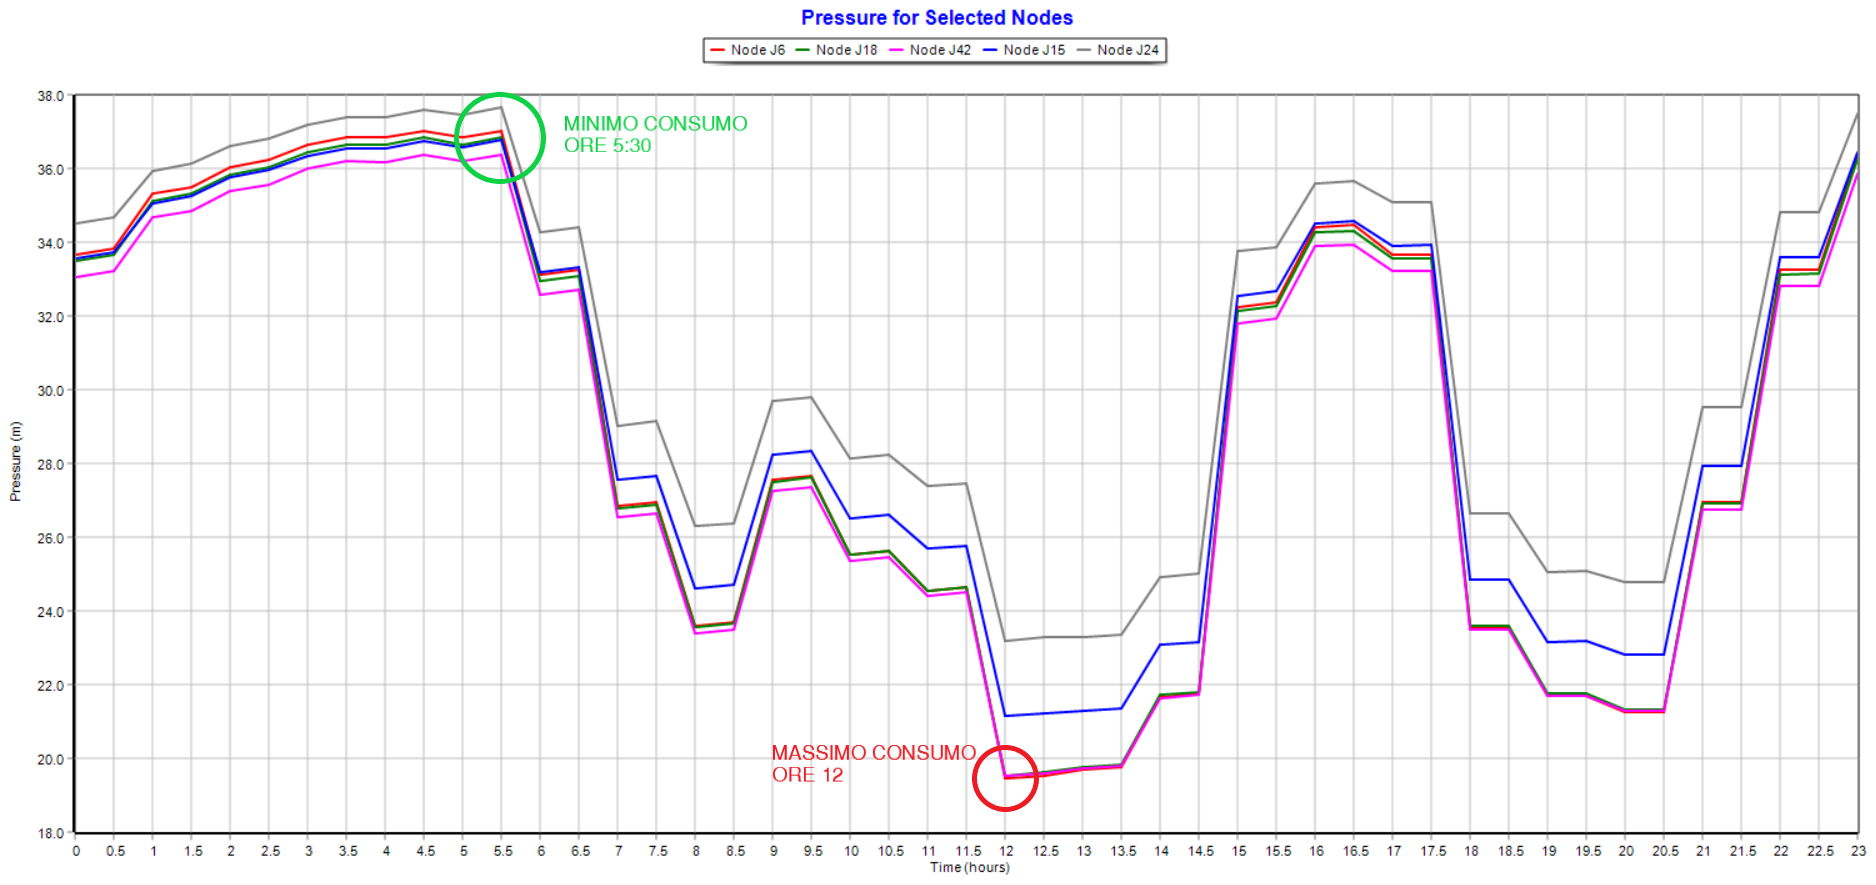
\includegraphics[width=\linewidth]{images/max-min_time}}
	   \onslide<2>\subfloat{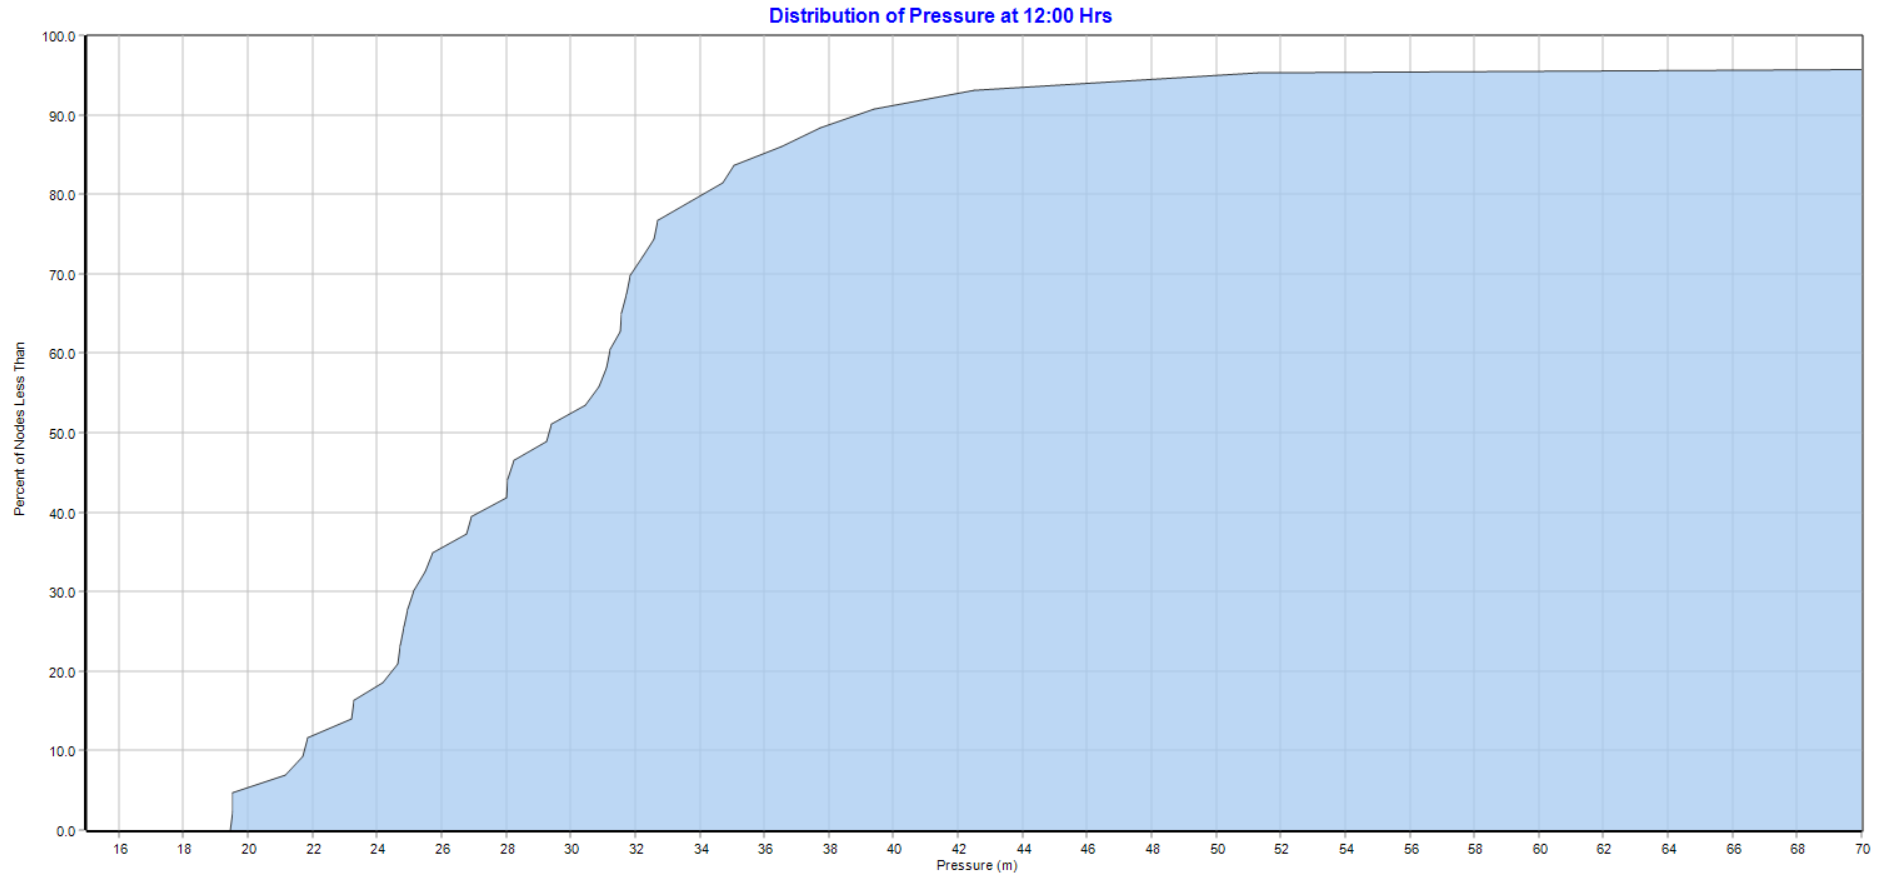
\includegraphics[width=\linewidth]{images/pressure_distribution_max_cons}}
	   \onslide<3>\subfloat{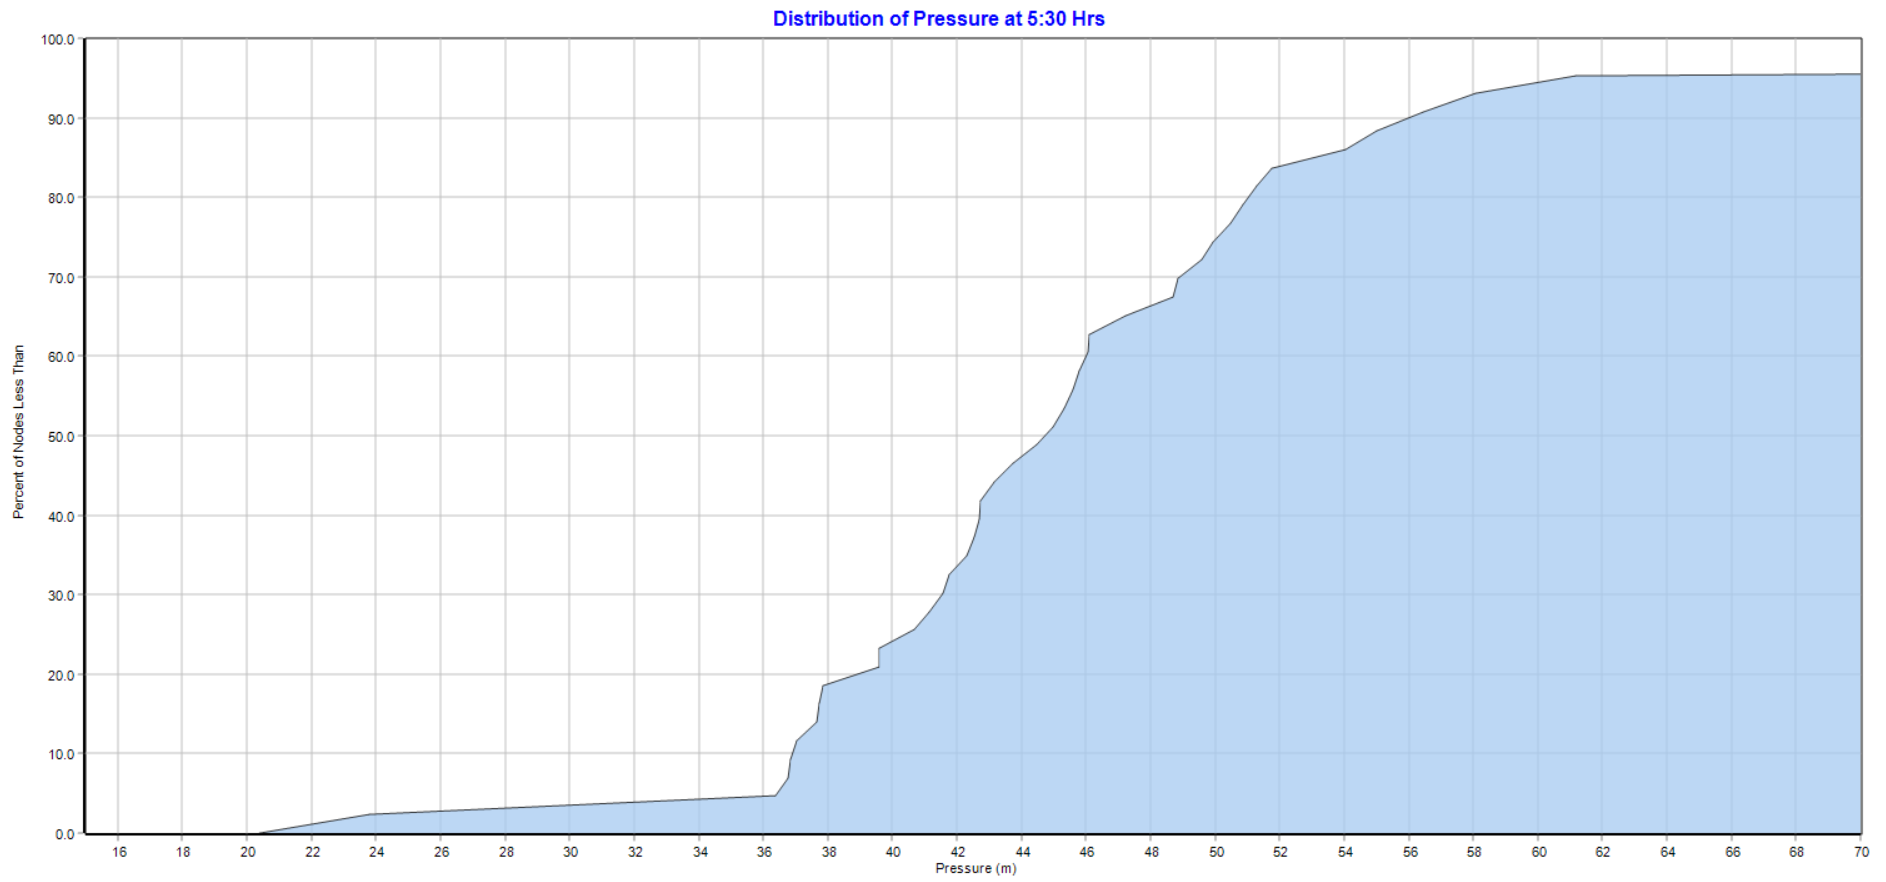
\includegraphics[width=\linewidth]{images/pressure_distribution_min_cons}}
	  \end{overprint}
	  \end{figure}
	 \end{column}
%
	\begin{column}{.5\textwidth}
		\begin{itemize}[<+->]
		\onslide<1>\item in questa configurazione, il massimo e il minimo consumo si hanno rispettivamente alle 12:00 e alle 5:30 del mattino
		\onslide<2>\item nelle ore di massimo consumo, la distribuzione delle pressioni risulta maggiore di $18\,m$ di colonna d'acqua per tutti i nodi della rete
		\onslide<3>\item nelle ore di minimo consumo, la percentuale di nodi con pressioni inferiori a $70\,m$ di colonna d'acqua è di oltre il $90\%$, fatta eccezione per nodi ausiliari (pompa, valvole, etc.)
		\end{itemize}
	\end{column}
 \end{columns}
\end{frame}
}
%
\begin{frame}
	\frametitle{Analisi su Epanet}
	\framesubtitle{Massimo consumo: ore 12:00}
	\begin{columns}
		\begin{column}{.7\textwidth}
				\begin{figure}
					\centering
					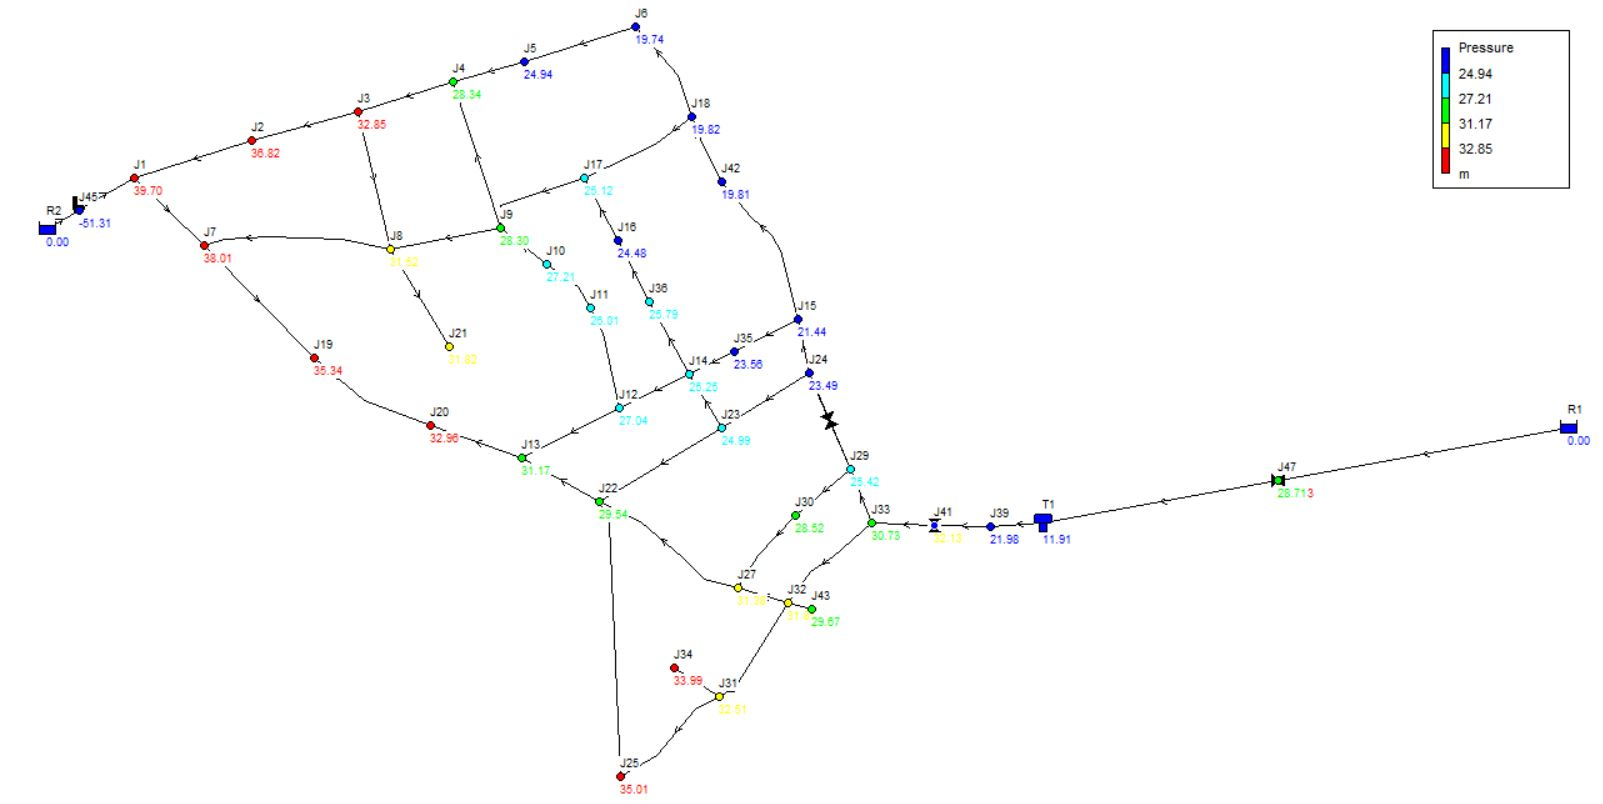
\includegraphics[width=\linewidth]{images/pressure_max_demand}
				\end{figure}
		\end{column}
%
		\begin{column}{.3\textwidth}
			\begin{align*}
				&\text{pressioni} \in [15, 70]\,m\\
				&\text{velocit\`a} < 2\,\dfrac{m}{s}
			\end{align*}
		\end{column}
	\end{columns}
\end{frame}
%
\begin{frame}
	\frametitle{Analisi su Epanet}
	\framesubtitle{Minimo consumo: ore 5:30}
	\begin{columns}
		\begin{column}{.7\textwidth}
				\begin{figure}
					\centering
					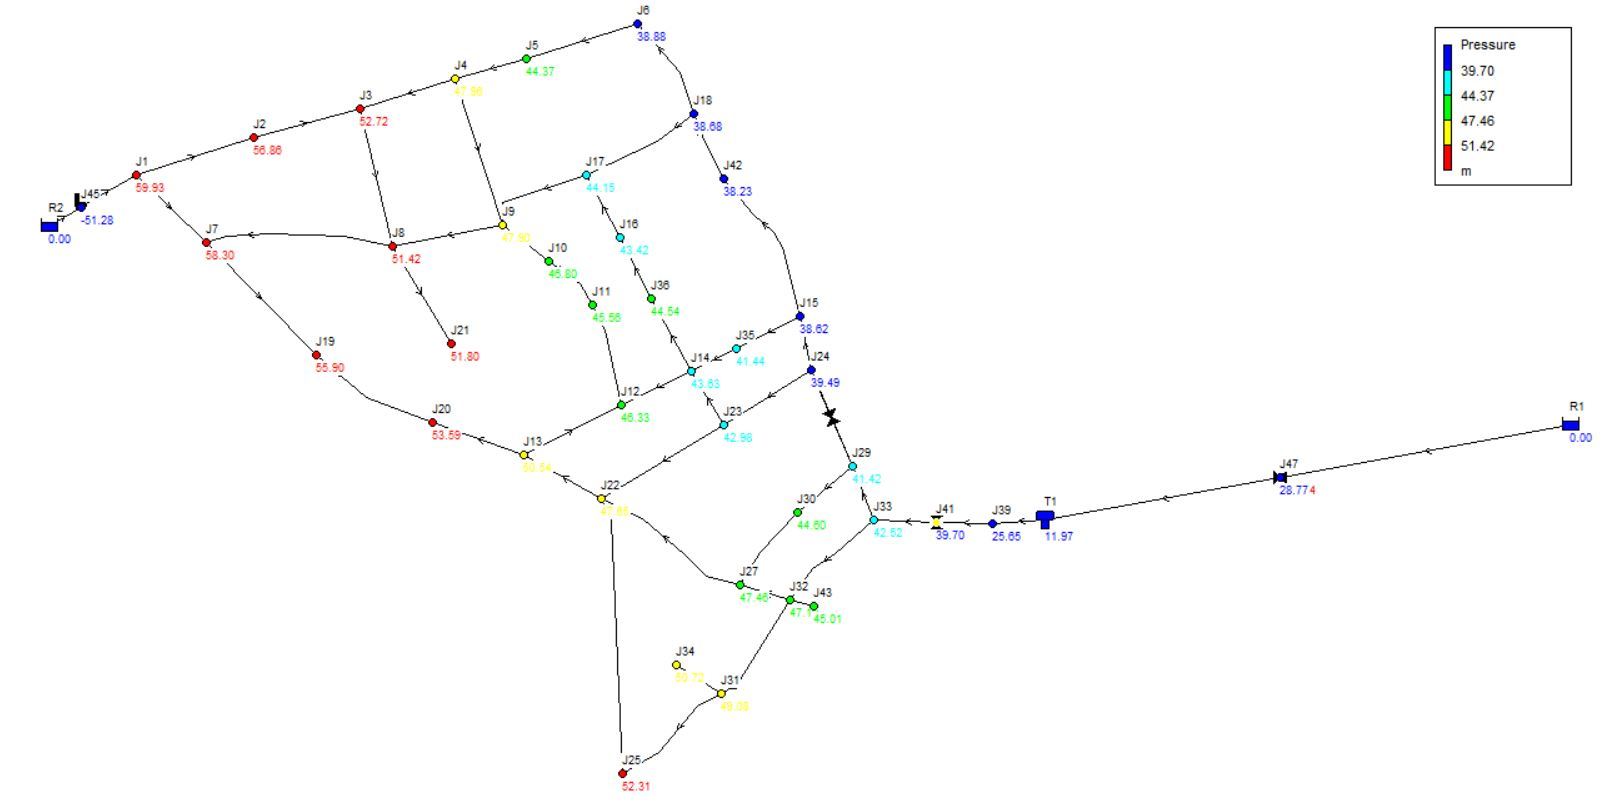
\includegraphics[width=\linewidth]{images/pressure_min_demand}
				\end{figure}
		\end{column}
%
		\begin{column}{.3\textwidth}
                $\text{pressioni} \in [15, 70]\,m$
                $\text{velocit\`a} < 2\,\dfrac{m}{s}$
		\end{column}
	\end{columns}
\end{frame}
%
%
%
{\nologo
\section{Analisi antincendio}
\begin{frame}
	\frametitle{Verifica antincendio}
	\begin{columns}
		\begin{column}{.7\textwidth}
				\begin{figure}
					\centering
					\begin{overprint}
						\onslide<1>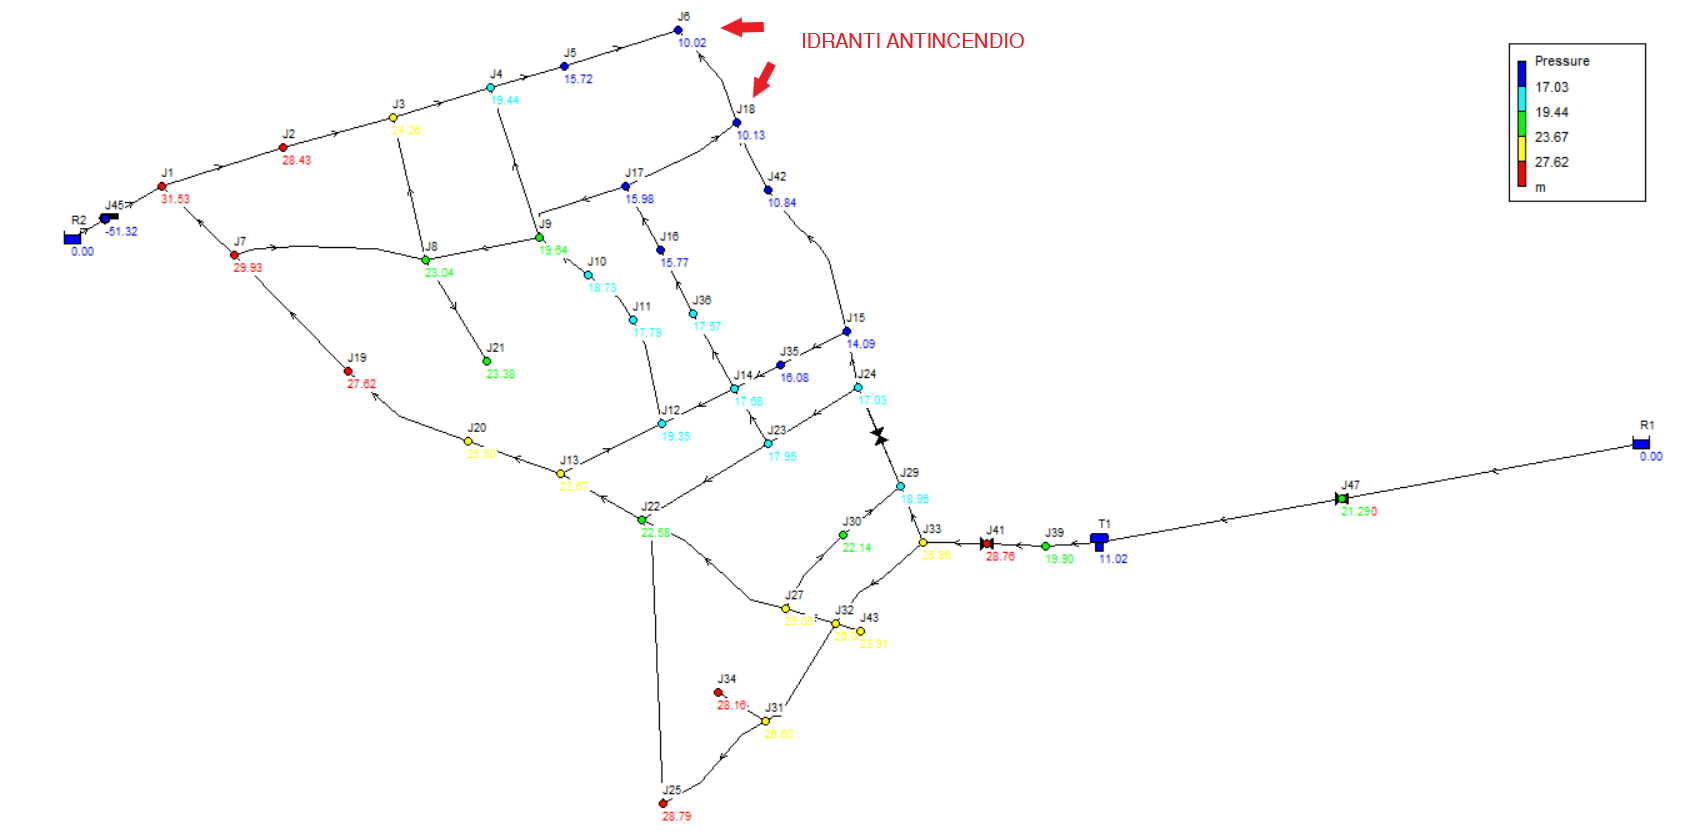
\includegraphics[width=\linewidth]{images/pressure_antincendio}
						\onslide<2>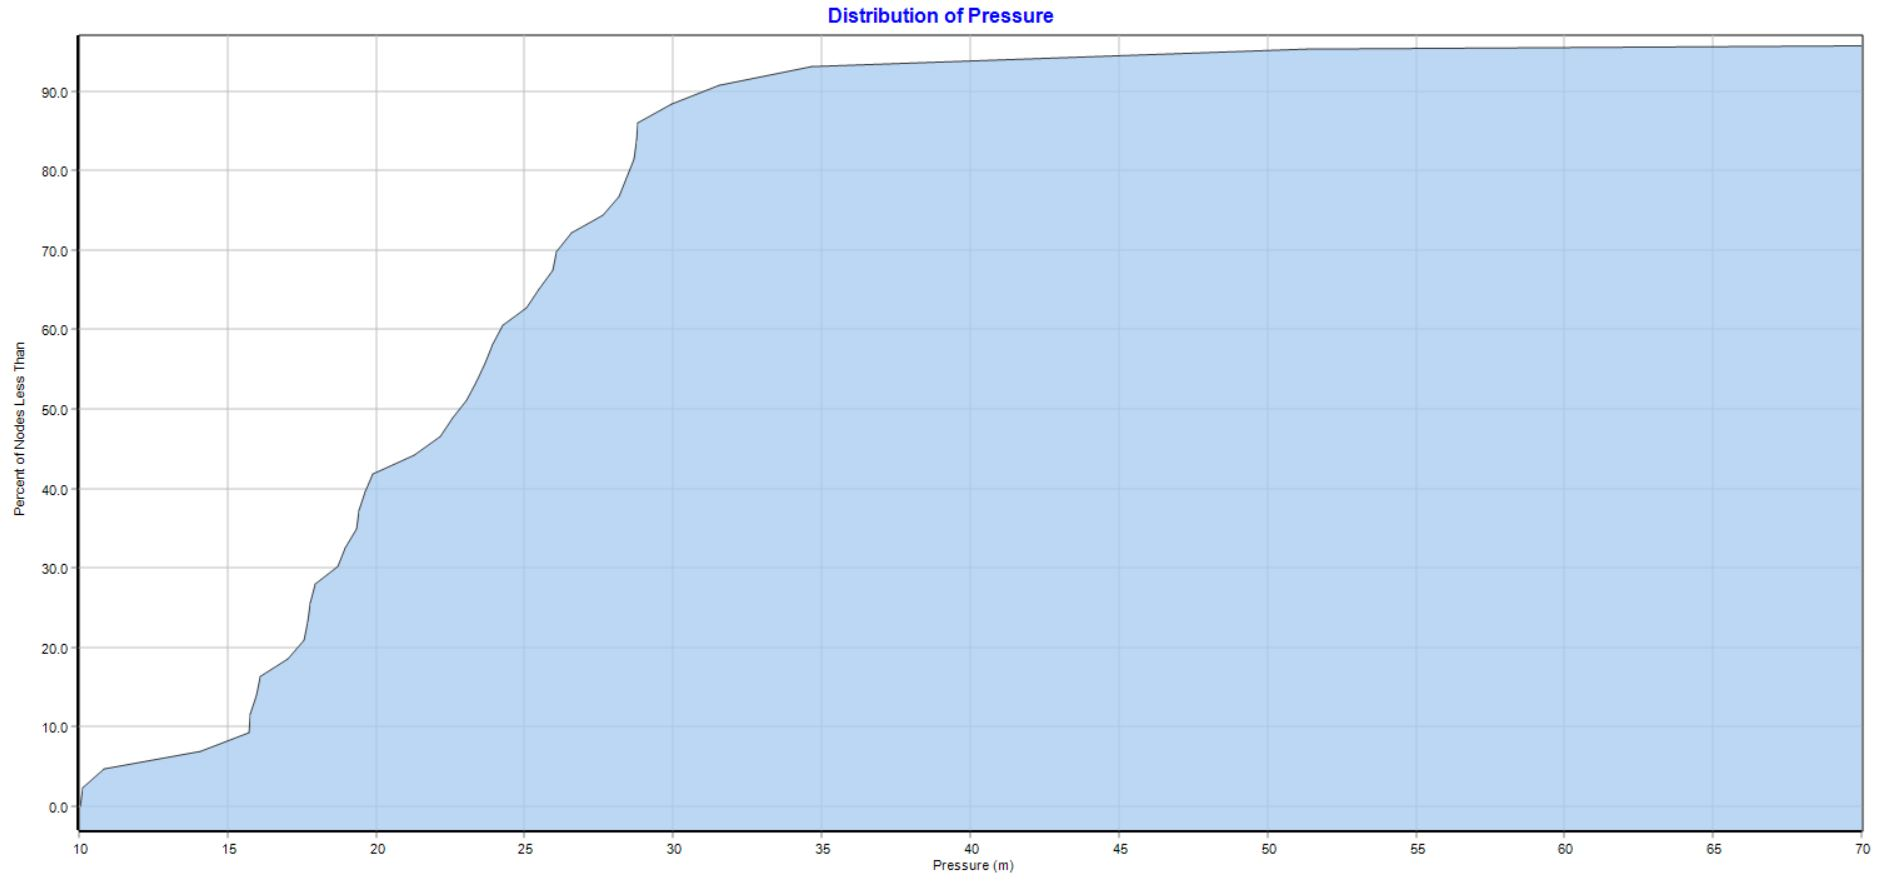
\includegraphics[width=\linewidth]{images/pressure_distribution_antincendio}
					\end{overprint}
				\end{figure}
		\end{column}
%
		\begin{column}{.3\textwidth}
			\begin{itemize}
				\onslide<1>\item n. 2 idranti
				\item portata supplementare di $5\,l/_s$ ai nodi critici per 1 ora
				\onslide<2>\item circa il 90\% dei nodi hanno carico $> 15\,m$
				\item tutti i nodi hanno carico $>10\,m$ sopra al piano stradale
			\end{itemize}
		\end{column}
	\end{columns}
\end{frame}
}
%
%
%
\section{Analisi rottura}
\begin{frame}
	\frametitle{Verifica alla rottura}
	\begin{columns}
		\begin{column}{.7\textwidth}
				\begin{figure}
					\centering
					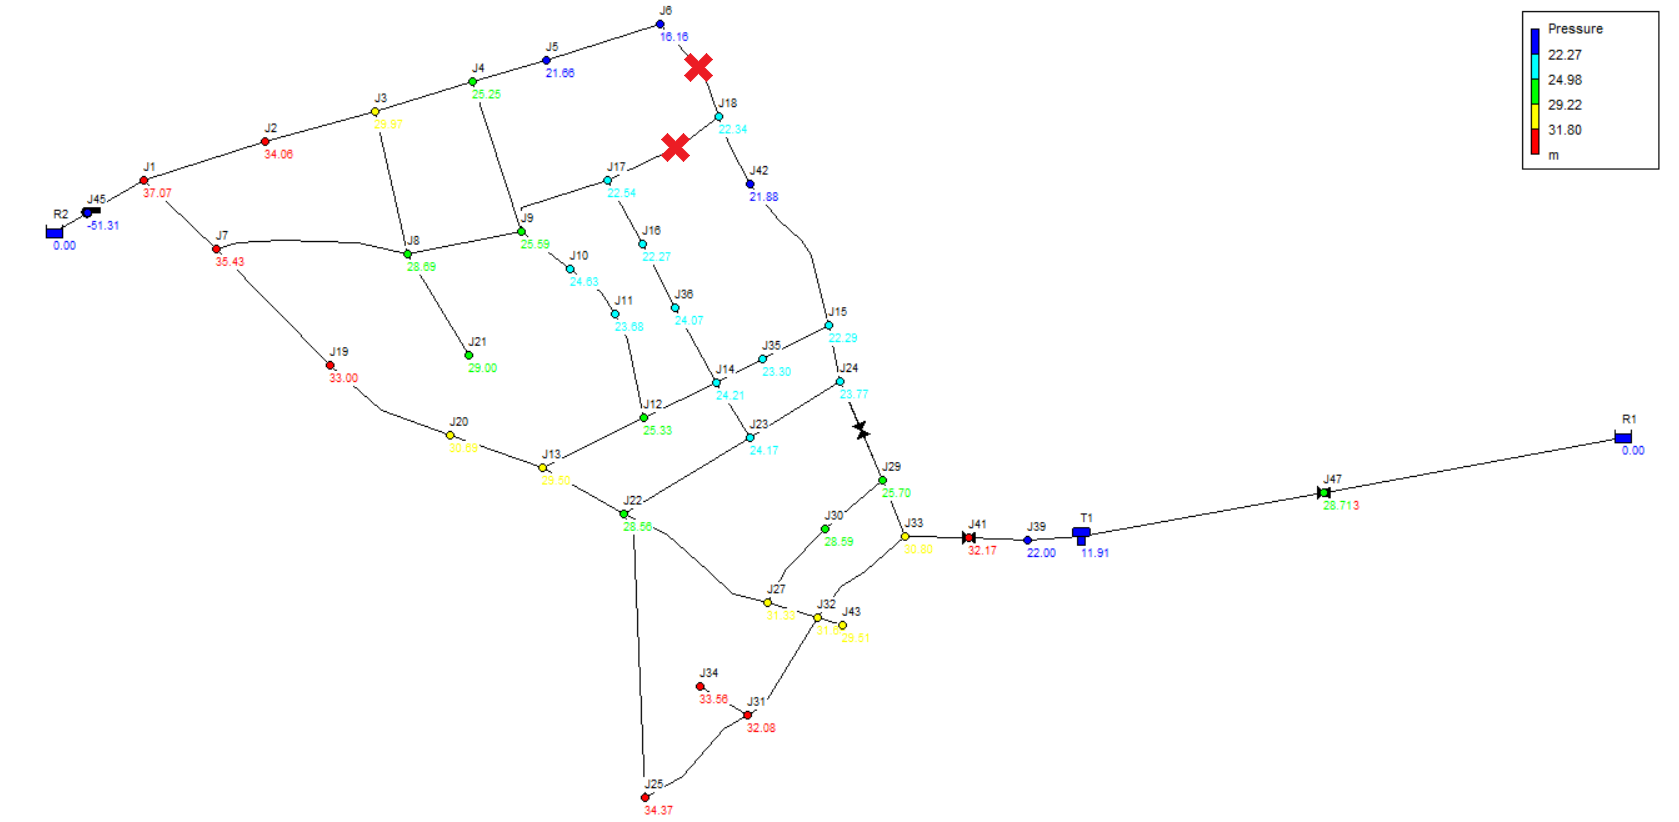
\includegraphics[width=\linewidth]{images/pressure_rottura}
				\end{figure}
		\end{column}
%
		\begin{column}{.3\textwidth}
			\begin{itemize}
				\item n. 2 rotture nella zona critica
				\item la rete è verificata
			\end{itemize}
		\end{column}
	\end{columns}
\end{frame}
%
%
%
\section{Computo metrico estimativo}
{\nologo
\begin{frame}
	\frametitle{Configurazione finale delle tubazioni}
	\begin{figure}
	 \centering
	 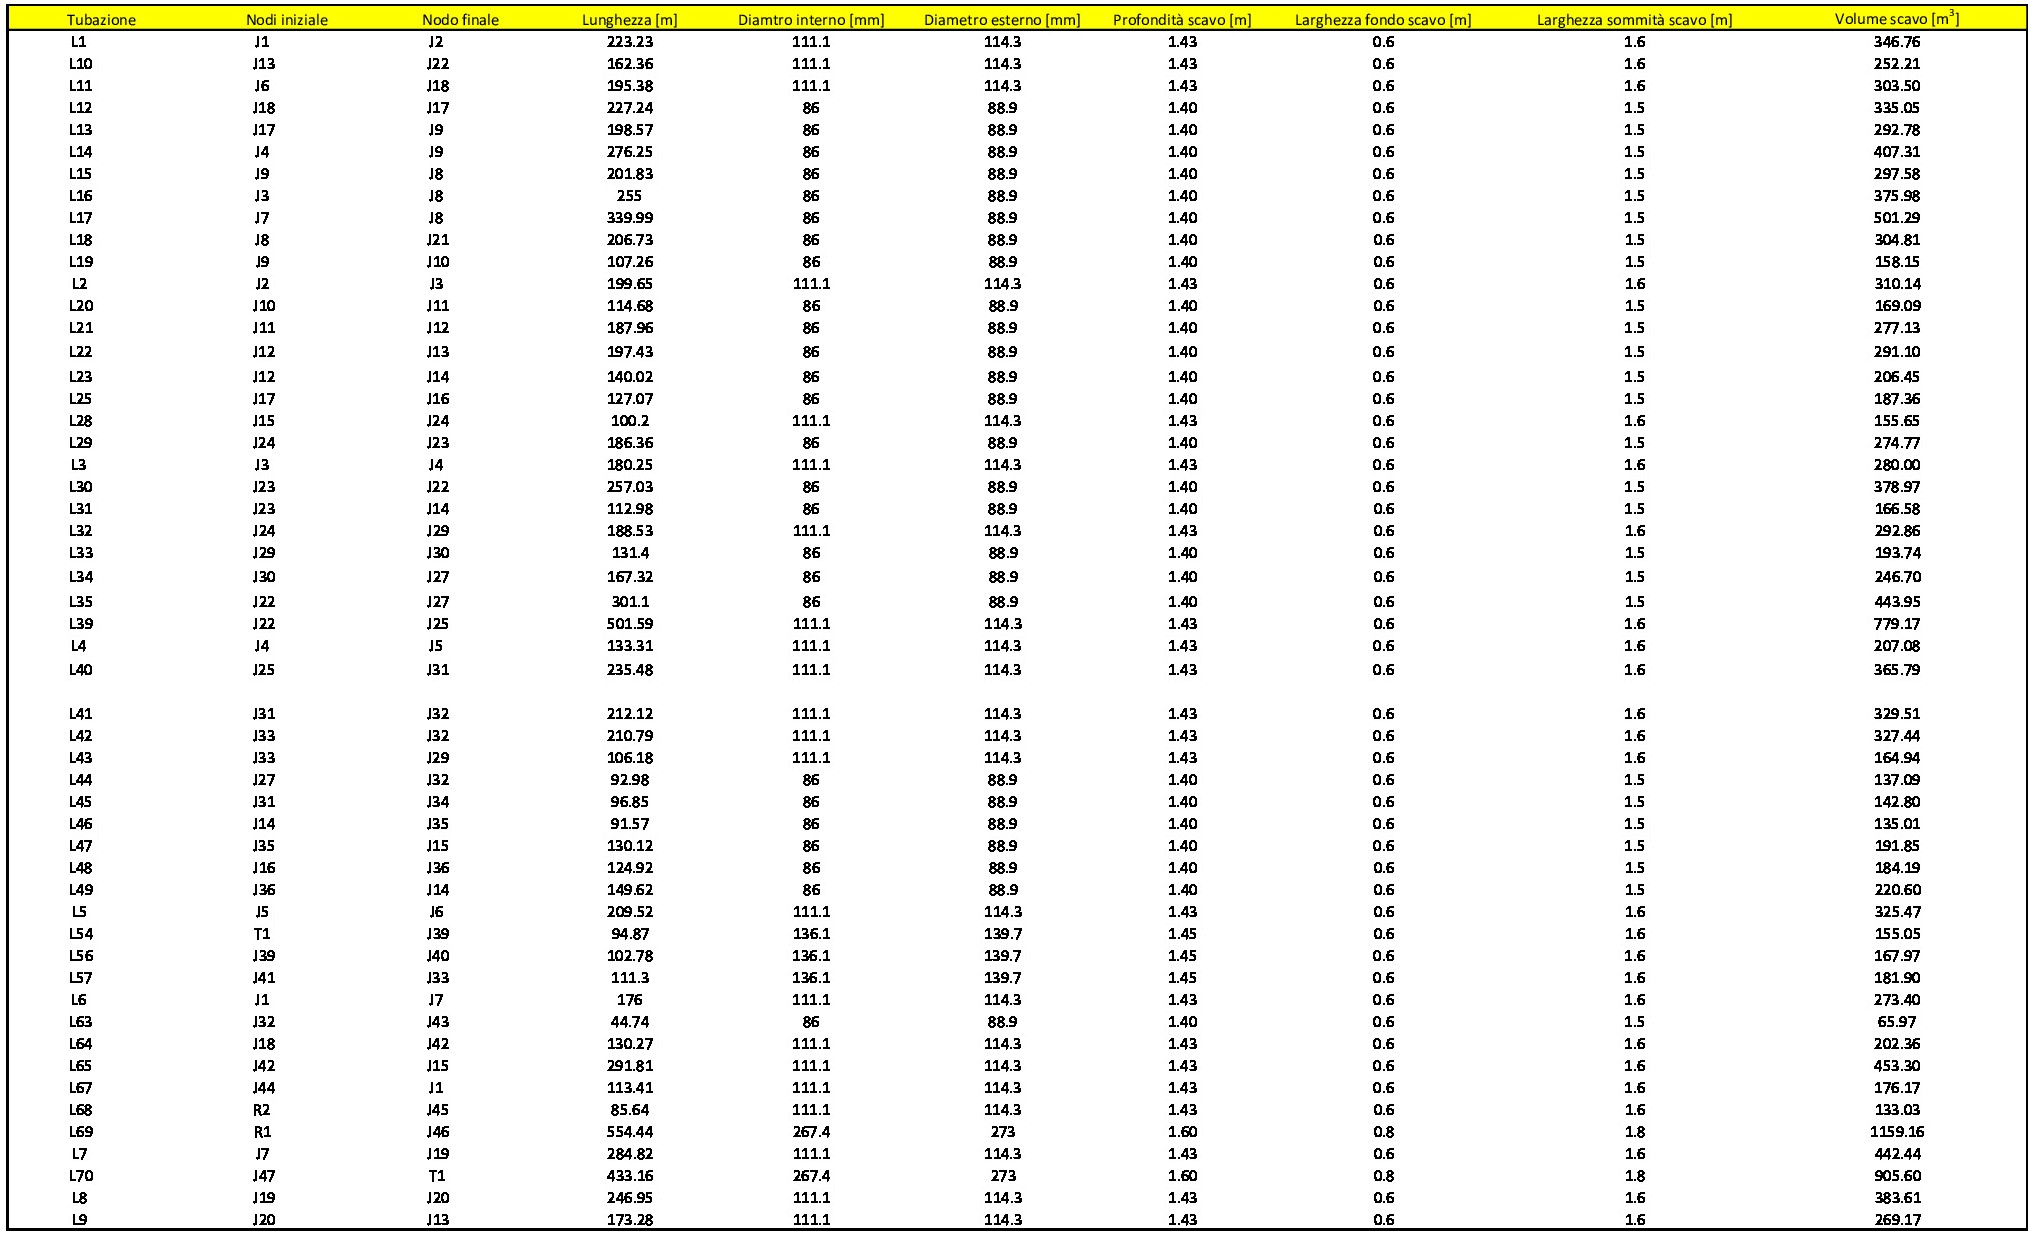
\includegraphics[width=\textwidth]{images/condotte}
	\end{figure}
\end{frame}
}
%
\begin{frame}
	\frametitle{Costo delle tubazioni}
	\framesubtitle{Costi derivanti dall'elenco prezzi della Provincia Autonoma di Trento}
	Fornitura e posa in opera di tubazioni in acciaio saldato bitumate
	\begin{figure}
	 \centering
	 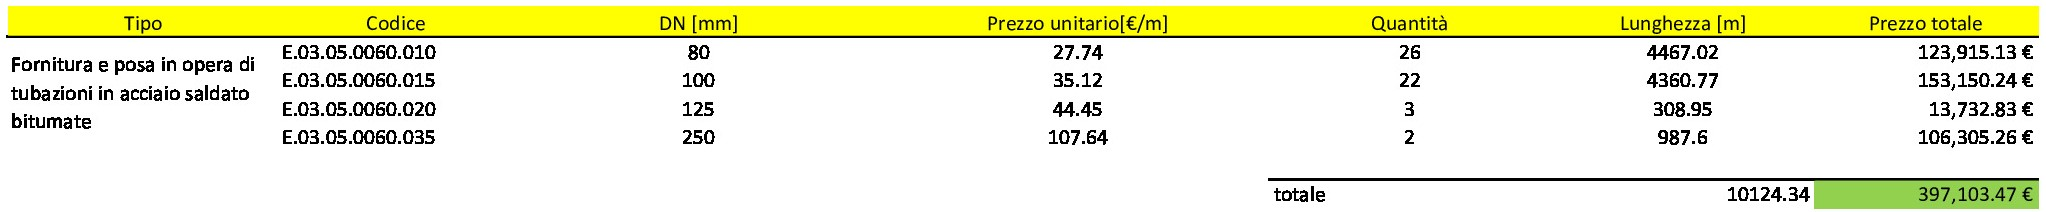
\includegraphics[width=\textwidth]{images/costo_condotte}
	\end{figure}
\end{frame}
%
\begin{frame}
	\frametitle{Costo dei pozzetti}
	\framesubtitle{Costi derivanti dall'elenco prezzi della Provincia Autonoma di Trento}
	Fornitura e posa in opera di fondo DN 120 per la realizzazione di pozzetto prefabbricato, in calcestruzzo vibro compresso, non armato, rinforzato con fibre di acciaio e con armature tradizionali, di forma interna circolare, con elemento di finitura ad incastro per la realizzazione di pozzetto prefabbricato, per l'accesso e l'aerazione fornito con guarnizione di tenuta incorporata conforme alle norme UNI EN 681.
	\begin{figure}
	 \centering
	 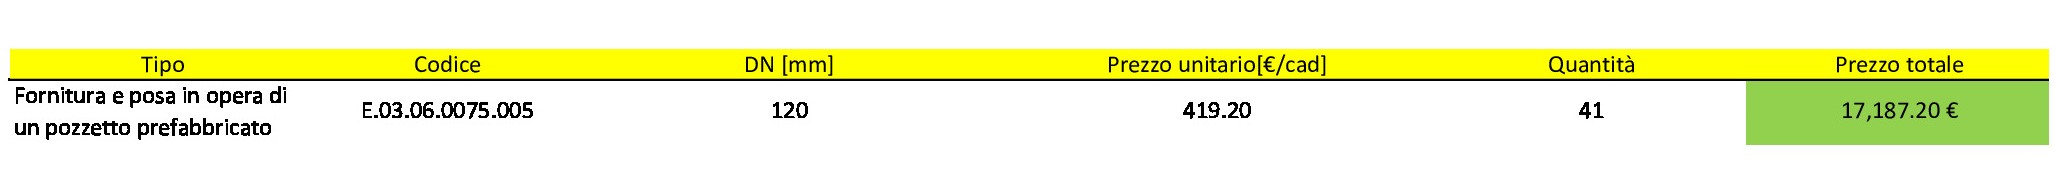
\includegraphics[width=\textwidth]{images/costo_pozzetti}
	\end{figure}
\end{frame}
%
{\nologo
\begin{frame}
	\frametitle{Costo dello scavo}
	\framesubtitle{Costi derivanti dall'elenco prezzi della Provincia Autonoma di Trento}
	Scavo a sezione ristretta, in terreno ordinario di qualsiasi natura e consistenza, anche in presenza d'acqua con tirante inferiore a $cm\,20$, eseguibile con mezzi meccanici, esclusa la roccia, compresi gli oneri [\dots] per la demolizione di pavimentazioni e sottofondi stradali di qualsiasi tipo non riutilizzabili, per la livellazione dei piani di scavo, per il deposito a fianco dello scavo del materiale, per il rinterro con materiale proveniente dagli scavi, [\dots]
	\begin{figure}
	 \centering
	 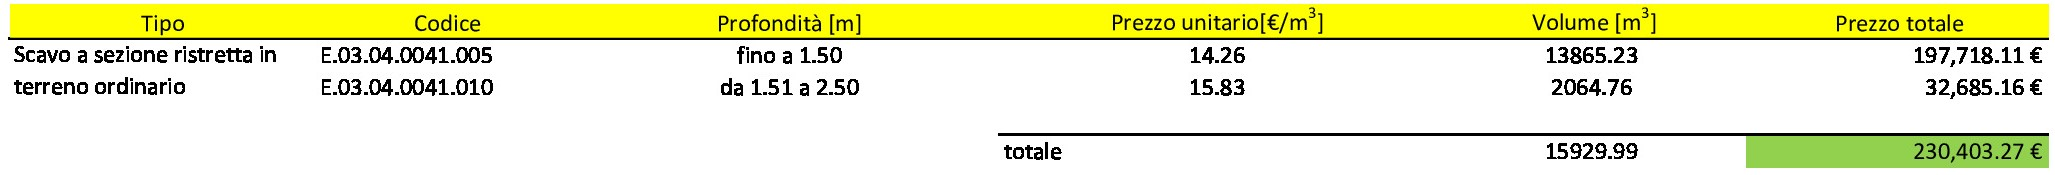
\includegraphics[width=\textwidth]{images/costo_scavo}
	\end{figure}
\end{frame}
}
%
\begin{frame}
	\frametitle{Costo dell'impianto di pompaggio}
	\framesubtitle{Costo derivante da \url{https://www.oppo.it/impianti/imp_pompa_somm_4.html}}
	Impianto di sollevamento su pozzo trivellato, profondità fino a 100 metri.\\
	Elettropompa sommersa centrifuga pluristadio $4"$ a giranti flottanti, camicia esterna, albero e testata in acciaio inox, motore 380V trifase, potenza $3\,kW$, raccordo filettato $1"\,1/4 F$
	\begin{figure}
	 \centering
	 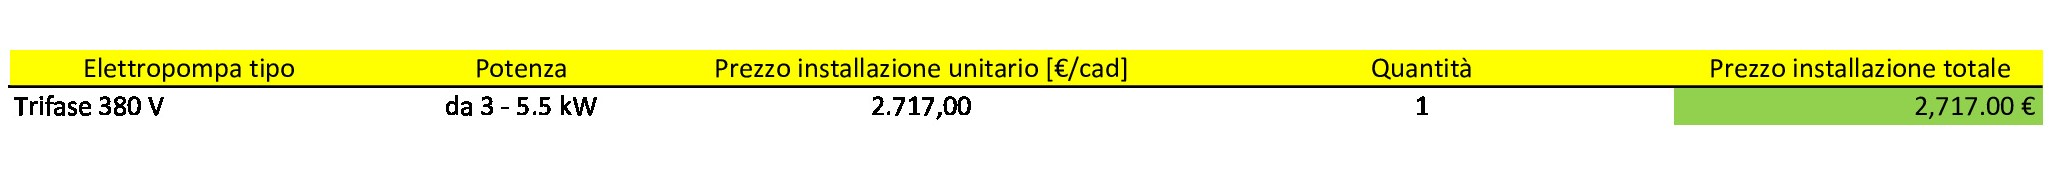
\includegraphics[width=\textwidth]{images/costo_impianto_pompa}
	\end{figure}
%
	\begin{figure}
	 \centering
	 \includegraphics[width=.5\textwidth]{images/costo_installazione_pompa}
	\end{figure}
\end{frame}
%
\begin{frame}
	\frametitle{Costo delle valvole}
	\framesubtitle{Costo derivante da \url{https://www.oppo.it/materiali/valvole/valvola_rid_press.html}}
	Valvola regolatrice di pressione a membrana
	\begin{figure}
	 \centering
	 \includegraphics[width=\textwidth]{images/costo_valvole}
	\end{figure}
%
	\begin{figure}
	 \centering
	 \includegraphics[width=.5\textwidth]{images/valves_oppo}
	\end{figure}
\end{frame}
%
\begin{frame}
	\frametitle{Costo totale dell'opera}
	Il costo totale dell’opera, tenendo conto anche di una percentuale del 5\% per gli imprevisti, risulta di
	\begin{figure}
	 \centering
	 \includegraphics[width=\textwidth]{images/costo_totale}
	\end{figure}
\end{frame}
%
\section{Fine}
{\nologo
	\usebackgroundtemplate{
		\tikz\node[opacity=.8] {\includegraphics[height=\paperheight]{images/acquedotto_sangano_valsusa.jpg}};}
	\begin{frame}
		\frametitle{Fine}
		\begin{center}
			\begin{minipage}{\textwidth}
				\begin{block}{}
				 \centering
				 \huge{Grazie per l'attenzione!}
				\end{block}
			\end{minipage}
		\end{center}
		
		\begin{tikzpicture}[overlay]%
			\node[xshift=-2.5cm,yshift=-3.4cm] at (current page.south east){\tiny{\color{white}{Acquedotto di Sangano in Val di Susa}}};
		\end{tikzpicture}

	\end{frame}
}
\end{document}
